\documentclass[a4paper,14pt]{report}
%\documentclass[a4paper,14pt]{extarticle}
\renewcommand{\baselinestretch}{1}
\renewcommand{\figurename}{Рисунок} 
\usepackage{ntheorem}

\usepackage[T2A]{fontenc}
\usepackage[utf8]{inputenc}
\usepackage[english,russian]{babel}
\usepackage{graphicx}
\usepackage{array}
\usepackage{tabularx}
\usepackage{setspace}

\usepackage{color}
\usepackage{url}
\usepackage{multicol}
\usepackage{amssymb}
\usepackage{hyperref}
%\usepackage[linesnumbered,boxed]{algorithm2e}
\usepackage{algorithm}
\usepackage{algpseudocode}
\usepackage{float}

\usepackage{longtable}
\usepackage{amsmath}
\usepackage{enumerate}
\usepackage{cancel}
\usepackage[justification=centering]{caption}
\usepackage{amsmath}


\newcommand{\ru}{\mathcal{R}_u}
\newcommand{\rt}{\mathcal{R}_i}
\newcommand{\R}{\mathcal{R}}
\newcommand{\rh}{\overline{\rho}}
\newcommand{\rhu}{\mathcal{\rho}_u}
\newcommand{\rhi}{\mathcal{\rho}_i}
\newcommand{\di}{\mathcal{\delta}_i}
\newcommand{\du}{\mathcal{\delta}_u}
\newcommand{\dc}{\mathcal{\delta}_c}
%\newcommand{\nip}{{\overset{i}{\mathcal{N}_p}}     }
%\newcommand{\nup}{{\overset{u}{\mathcal{N}_p}}     }
%\newcommand{\nit}{{\overset{i}{\mathcal{N}_{topN}}}}
%\newcommand{\nut}{{\overset{u}{\mathcal{N}_{topN}}}}
%\newcommand{\ec}{{\overset{c}{\mathcal{E}}}}
%\newcommand{\eap}{{\overset{a}{\mathcal{E}_{p}}}}
%\newcommand{\eat}{{\overset{a}{\mathcal{E}_{topN}}}}
%\newcommand{\eit}{{\overset{i}{\mathcal{E}_{topN}}}}
%\newcommand{\res}{\overline{T}^a_{\bot}}
\newcommand{\test}{T^a_{\bot}}
\newcommand{\midel}{\overline{\Delta}_{\rho}}


\theoremstyle{plain}
\newtheorem{myproof}{Доказательство}

%% \newtheorem{thm}{Theorem}[section]
%% \newtheorem{lem}[thm]{Lemma}
%% \newtheorem{prop}[thm]{Proposition}
%% \newtheorem*{cor}{Corollary}

% \theoremstyle{plain}
%% \newtheorem{thm}{Theorem}[section]
%% \newtheorem{lem}[thm]{Lemma}
%% \newtheorem{prop}[thm]{Proposition}
%% \newtheorem*{cor}{Corollary}

% \theoremstyle{definition}
%\setcounter{section}{0}
%% \newcommand{\mychapter}[1]{
%%     \setcounter{chapter}{#1}
%%     \setcounter{section}{1}
%%     \chapter*{#1}
%%     \addcontentsline{toc}{chapter}{#1}
%% }
%% \newcounter{assert}[subsection] 
%% \newcommand{\a}{\par \addtocounter{assert}{1}% 
%% \textbf{Утверждение \arabic{zadacha}}} 

\renewcommand{\thesubsection}{\thesection\arabic{subsection}}
%% \newtheorem{defn}{Определение}{indent}%[thesubsection]

\theoremstyle{break}
\newtheorem{assert}{Утверждение}
\newtheorem{assertSRS}{Утверждение СРС}
\newtheorem{assertORS}{Утверждение ОРС}
\newtheorem{assertNON}{}

%% \newtheorem{assert-plain}{indent}{Утверждение}%[thesubsection]
\newtheorem{exmp}{Example}%[thesection]

% \usepackage{alltt}
%% \makeatletter
%% \renewcommand{\@biblabel}[1]{#1.} % СпиСОМ литературы: `[1]' => `1.'
%% \makeatother
\renewcommand{\contentsname}{Оглавление}
%% % \theoremstyle{plain}% default
%% \newtheorem{thm}{Теорема}
%% \newtheorem{ax}{Аксиома}
%% \newtheorem{prop}{Доказательство Теоремы}
%% \@addtoreset{equation}{section} % Счетчик формул

% \tableofcontents
%\usepackage{geometry} % Меняем поля страницы
%\geometry{left=2.2cm}% левое поле
%\geometry{right=2.2cm}% правое поле
%\geometry{top=1.9cm}% верхнее поле
% Чтобы убрать Гадава N
\makeatletter
\def\@makechapterhead#1{%
  \vspace*{30\p@}%
  {\parindent \z@ \raggedright \normalfont
    \interlinepenalty\@M
    \large \bfseries #1\par\nobreak
    \vskip 40\p@
  }}
\def\@makeschapterhead#1{%
  \vspace*{30\p@}%
  {\parindent \z@ \raggedright
    \normalfont
    \interlinepenalty\@M
    \large \bfseries  #1\par\nobreak
    \vskip 20\p@
  }}
\makeatother


\begin{document}
\begin{titlepage}
\begin{center}
\textsc{}\\
\end{center}
\vspace{1.5cm}
\begin{flushright}
{\it На правах рукописи}
\end{flushright}
\vspace{3.5cm}
\begin{center}
{Понизовкин Денис Михайлович}
\par
\vspace{2cm}
\textsc{
МАТЕМАТИЧЕСКАЯ МОДЕЛЬ РЕКОМЕНДАТЕЛЬНОЙ СИСТЕМЫ НА НЕЧЕТКИХ МНОЖЕСТВАХ КАК
	ЭФФЕКТИВНОЕ РАСШИРЕНИЕ АНАМНЕСТИЧЕСКИХ КОЛЛАБОРАТИВНЫХ МОДЕЛЕЙ
	}
\par
\vspace{2cm}
{05.13.17 --- Теоретические основы информатики}
\par
\vspace{2cm}
{Автореферат\\
диссертации на соискание ученой степени\\
кандидата технических наук}
\end{center}
\par
\vspace{3.5cm}
\begin{center}
%{Нижний Новгород\\
%2016}
\end{center}
\end{titlepage}

%% \thispagestyle{empty}
%% {Работа выполнена на кафедре БЕЗсистемного программирования ма\-те\-ма\-ти\-ко-ме\-ха\-ни\-чес\-ко\-го
%% факультета Санкт-Петербургского государственного университета.

%% \vspace{0.8cm}

%% \begin{tabbing}
%% Научный руководитель:\quad\quad\=доктор физико-математических наук,\\
%% \quad\>проф. ЛЬВОВ Гепард Тигранович\\
%% \>\\
%% Официальные оппоненты:\>доктор физико-математических наук,\\
%% \quad\>проф. ПРЕОБРАЖЕНСКИЙ Филипп Филиппович\\
%% \quad\>(ОАО \lquot НИИЧАВО\rquot, Москва)\\
%% \>\\
%% \>кандидат физико-математических наук,\\
%% \quad\>ЧУДАКУЛЛИ Наверн Орландович\\
%% \quad\>(Unseen University, Анк-Морпорк)\\
%% \>\\
%% Ведущая организация:\>Институт благородных девиц\\
%% \quad\>(Смоленск)\\
%% \>
%% \end{tabbing}


%% \vspace{0.8cm}
%% \noindent Защита диссертации состоится ``\underline{\phantom{332}}''\underline{\phantom{xxxxxxxxxx}} 1889 года
%% в \underline{\phantom{25}} часов на заседании совета Д212.232.51 по защите
%% докторских и кандидатских диссертаций при Санкт-Петербургском государственном университете по адресу: 198504, Санкт-Петербург, Петродворец, Университетский пр., д.~28, математико-механический факультет, ауд. 3В.

%% \vspace{0.8cm}
%% \noindent С диссертацией можно ознакомиться в Научной библиотеке Санкт-Пе\-тер\-бург\-ского государственного
%% университета по адресу: 199034, Санкт-Петербург, Университетская наб., д.~7/9.

%% \vspace{0.8cm}
%% Автореферат разослан ``\underline{\phantom{332}}''\underline{\phantom{xxxxxxxxxx}} 1889 года.

%% \vspace{2.5cm}
%% \noindent Ученый секретарь\\
%% диссертационного совета\\
%% доктор физико-математических наук,\\
%% профессор\phantom{xxxxxxxxxxxxxxxxxxxxxxxxxxxxxxxxxxxxxx}Перфокартов. И. К.
%% }
%% \end{document}



% \tableofcontents

%% \begin{center}
%% ОБЩАЯ ХАРАКТЕРИСТИКА РАБОТЫ
%% \end{center}
\begin{center}
ОБЩАЯ ХАРАКТЕРИСТИКА РАБОТЫ
\end{center}


{\bf Актуальность работы и степень разработанности.}
С интенсивным развитием веб-технологий, огромным и постоянно растущим числом
информации, доступной через интернет с помощью множества различных устройств,
популярными становятся рекомендательные системы (далее РС), которые облегчают
пользователю задачу поиска нужной информации путем рекомендации такой информации
или путем определения степени близости конкретной информации пользователю.

Исходные данные РС --- множество
$P := \{(u, i, \rho(u, i)): \rho(u, i) \ne \bot\}$,
где символ $\bot$ означает неизвестное значение, и:
\begin{itemize}
	\item $u \in U := \{1,...,m\}$ --- идентификаторы пользователей РС;

	\item $i \in I := \{1,...,n\}$ --- идентификаторы объектов предметной
области РС. Например, объектом может фильм кинематографической РС.
Для простоты изложения не будем каждый раз употреблять выражение
<<идентификатор пользователя или объекта>>, а будем обозначать коротко
<<пользователь или объект>>;

	\item $\rho: U \times I \rightarrow \{[0,1] \bigcup \bot\}$ --- функция оценки близости
		пользователей и объектов. Значение $\rho(u,i)$ показывает, насколько
		объект $i$ по своим характеристикам близок предпочтениям пользователя $u$.
		Как правило, оценки близости задаются самими пользователями во время
		работы с РС.
		Будем считать, что чем меньше значение оценки, тем объект ближе.
		Будем говорить, что между пользователем $u$ и
		объектом $i$ выполняется отношение близости $\R$, если
		$\rho(u, i) \le \varepsilon_{\R}$, где $\varepsilon_{\R} \in [0,1]$ --- некоторая
		малая фиксированная величина.
		Будем называть таких пользователей и объектов близкими.
	\end{itemize}

Зачастую в исследованиях РС исходные данные
представляются в виде матрицы, элементами которой являются
значения $\rho(u, i)$. Как правило, если $\rho(u, i) \ne \bot$,
то это значение задал сам пользователь за время работы с системой
(к примеру, поставил оценку фильму):

\begin{center}
$\mathcal{M}_{\rho} =
\begin{pmatrix}
	\rho(1,1)& ... & \rho(1,n)  \\
	...      & \bot & ...  \\
	\rho(m,1)& ... & \rho(m,n)  \\
\end{pmatrix}$.\\
\end{center}

Матрица
$\mathcal{M}_{\rho}$ является разреженной, то есть большинство
значений \\ $\rho(u, i) = \bot$.
Разреженность матрицы $\mathcal{M}_{\rho}$ является причиной
существования проблемы поиска нужной информации, иначе от системы требовалось
бы только выбрать подмножества объектов с заданной оценкой близости. Эта же
причина послужила толчком для
возникновения и развития РС как инструмента, способного снизить степень
разреженности для каждого пользователя (называемого в таком случае активным
и обозначаемого символом $u_a$) путем решения следующих двух задач:
\begin{enumerate}
	\item прогнозирования (обозначим как $pred$). По данной задаче требуется
		спрогнозировать неизвестное значение $\rho(u_a, i_{\bot})$.
		Спрогнозированное значение будем обозначать символов $\rh(u_a,
		i_{\bot})$.

\item $topN$. По данной задаче требуется сформировать подмножество объектов
	$I_{topN} = \{i: (u_a \R i) \wedge \rho(u_a, i) = \bot\}
		\wedge |I_{topN}| = N \le n$.
		%Так как неизвестно, выполняется
		%ли отношение $u_a \R i$ в силу того, что $\rho(u_a, i) = \bot$,
		%то выполнение отношения $u_a \R i$ определяется по значению
		%прогнозной функции: $u_a \R i \Leftrightarrow \rh(u_a, i) <
		%\varepsilon_{\R}$.
\end{enumerate}

%Разнообразие существующих оценок приводит к проблеме выбора той или иной
%оценки для определения качества полученных результатов. Некоторые исследователи
%вводят свои собственные показатели качества. Проблематично сравнивать
%результаты различных исследований и невозможно сравнить результаты решений
%задачи $topN$ и $p$.
%Отсутствие стандартизации оценок приводит к проблеме интеграции знаний в области
%РС и наносит ущерб их прогрессу. Данные проблемы были определены Дж. Херлокером.

Существуют различные математические модели РС,
которые задают способ
представления данных о пользователях и объектах и
методы решения задач.
В диссертации исследуется одна из самых известных,
хорошо изученных
	\footnote{Recommender Systems in Computer Science and Information Systems
	--- A Landscape of Research / D. Jannach, M. Zanker, M. Ge [и др.]
	// International Conference on Electronic Commerce and Web Technologies.
	2012. С. 76–87.}
моделей РС --- анамнестическая коллаборативная модель
РС (далее АКМ). АКМ является одним из классов
коллаборативных моделей, применяющих методы коллаборативной фильтрации.
Методы решений задач АКМ используют анамнестические алгоритмы, которые
основаны на аксиомах, являющихся эвристическимb утверждениями
	\footnote{
		Toward the next generation of recommender systems: A survey of the
		state-of-the-art and possible extensions / G Adomavicius, A Tuzhilin //
		IEEE transactions on knowledge and data engineering. Т. 17, С 734-749

		Umyarov A., Tuzhilin A. Improving Collaborative Filtering Recommendations
		Using External Data // ICDM ’08 Proceedings of the 2008 Eighth IEEE
		International Conference on Data Mining. 2008. С. 618–627.

		Wang Jun. Unifying user-based and item-based collaborative filtering approaches
		by similarity fusion // SIGIR ’06 Proceedings of the 29th annual international
		ACM SIGIR. 2006.

		Berkovsky S., Kuflik T., Ricci F. Cross-Domain Mediation in Collaborative
		Filtering // Proceedings of the 11th international conference on User Modeling.
		2007. С. 355–359.
	}.
РС, использующие АКМ, внедрены во многие известные веб-сервисы:
Amazon, Netflix, IMDB, Kinopoisk, LastFm и т.д.
Изучением коллаборативной фильтрации занимались такие известные исследователи как
Г. Адамовичус, Дж. Констан, Дж. Карипис, Г. Ф. Рикки, Г. Ву, Л. Рокач, Б. Сарвар, А. Тужилин, Б. Шапираи, Дж. Херлокер и др.
Несмотря на успешность, популярность, заявляемую разработанность методов
коллаборативной фильтрации, на то,
что эти методы были интегрированы в бизнес более пятнадцати лет назад,
и на то, что они
уже стали называться Г. Адамовичиусом, А. Тужилиным, М. Экстрандом,
Дж. Ридлом и Дж. Констаном традиционными,
существует ряд открытых актуальных проблем, связанных с их применением.

% Чтоб не докопались
% Из Recommender System for an IPTV Service Provider
% Content-based systems [1, 3, 21] recommend items similar to those that a user
% liked in the past, by considering their features 

% item based
%Item-Based Top-N Recommendation Algorithms
%The primary motivation behind these algorithms is the fact
%that a customer is more likely to purchase items that are similar to the items
%that he/she has already purchased in the past; thus, by analyzing historical
%purchasing information (as represented in the user–item matrix) we can automatically identify these sets of similar items and use them to form the top-N
%recommendations. %
%
% model based
%Evaluation of item-based top-N recommendation algorithms 
%In this paper we present one such class of model-based
%top-N
%recommendation algorithms. These algorithms first
%determine the similarities between the various items and then used them to identify the set of items to be recommended.%
%
%

%Одной из проблем является отсутствие единых теории, терминологии и
%обозначений АКМ. К примеру, один и тот же метод, заключающийся в фильтрации
%объектов, носит различные наименования: объектно-ориентирован-ный (например, в
%работе <<Item-Based Top-N Recommendation Algorithms>>)
%модельный (например, в работе <<Evaluation of item-based top-N recommenda-tion algorithms>>),
%контентный (например, в работе <<Recommender System for an IPTV Service
%Provider>>).

%Существующие исследования носят, в основном, эмпирический характер,
%и анализ причин, почему один и тот же метод хорошо работает на одних данных, а
%на других --- нет, не проводится.

Для того, чтобы описать существующие проблемы,
введем понятие эффективности модели.
Будем говорить, что модель РС эффективна по некоторому критерию, если она
удовлетворяет ему независимо от дополнительных условий и ограничений.
В работе рассматриваются три критерия эффективности РС: (1) качество
решения, (2) вычислительная сложность и (3) стабильность, где стабильностью
будем называть свойство системы решать задачу качественно независимо
от исходных данных.

Чтобы определить эффективность по критерию качества или стабильности
проводится тестирование. Для этого исходное множество данных $P$
разбивается на обучающее и тестовое множества, которые обозначим символами
$P_0$ и $P_{\bot}$ соответственно.
Если $(u, i, \rho(u, i)) \in P_0$, то будем обозначать такие объекты $i_0$.
Если $(u, i, \rho(u, i)) \in P_{\bot}$, то будем обозначать такие объекты $i_{\bot}$.
После получения результирующего множества
$\overline{P}_{\bot} = \{(u, i, \rh(u_a, i))\}$ в ходе решения задачи
по данным обучающего множества, проводится
сравнение результирующего множества с тестовым. Сравнение производится
с помощью функций, называемых оценками качества. Для каждой задачи существует
своя группа оценок, в которую входит некоторое число функций. Например,
некоторые из оценок задачи $pred$ --- это MAE, NMAE, RMSE,
из оценок задачи $topN$ --- точность P, точность P@L по списку длины L, средняя точность
P@L, NDCG.
Будем говорить, что решение задачи $t$ эффективно по критерию качества,
если $\mathcal{E}_{t}(\overline{P}_{\bot}, P_{\bot}) \le \varepsilon_{t},$ где
$t \in \{topN, pred\}$, $\mathcal{E}_{t}$ --- оценка качества
решения задачи $t$, $\varepsilon_{t} \in [0,1]$ --- некоторая фиксированная
величина.
%В диссертации исследуются используемые оценки решения и двумерные
%РС, а, точнее, их самые известные представители --- коллаборативные РС (далее
%КМ). Эти системы основаны на коллаборативной фильтрации.
Как говорилось выше, АКМ основаны на эвристических утверждениях.
Выполнение эвристических утверждений в существующих исследования
не рассматривается, но оно обусловлено свойствами исходных данных.
Если исходные данные обладают свойствами динамики или неоднородности, то
эвристические утверждения не выполняются. А, так как на них базируются методы
решений задач, то нет гарантии получения эффективного решения по критерию
качества на любых исходных данных, или на одних
и тех же данных, но меняющихся со временем. Поэтому коллаборативные модели
не являются эффективными по критерию стабильности. Реальные данные, как
правило, обладают и тем и другим свойством. Зависимость качества решения
от свойств исходных данных приводит к тому,
что конкретная реализация РС эффективна по критерию качества на определенных
данных или в определенный момент времени,
но может быть неэффективной на других данных или в следующий момент времени.
Поэтому не существует более или менее универсальной модели, которую можно
применять в различных предметных областях, а существующие модели с течением
времени требуют внесения доработок.
%и требует доработки и дополнительной настройки,
%для чего необходимо выделять дополнительные ресурсы.

%На эвристических утверждениях базируется оценка задачи
%$topN$, поэтому, если исходные данные обладают свойством динамики или
%неоднородности, то значение оценки $\mathcal{E}_{topN}$ не является объективным
%показателем. Поэтому становится невозможным объективно оценивать те или иные
%подходы, применяемые в решении задачи $topN$.

Если исходные данные таковы, что эвристические утверждения выполняются,
то получение эффективного решения по критерию качества
ограничено дополнительными условиями, зависящими от применяемых
мер сходства, выбор которых производится разработчиками АКМ.
В общем же случае дополнительные условия не выполняются, поэтому АКМ
не эффективны по критерию качества.

Алгоритмы решения задач АКМ имеют высокую асимптотическую сложность.
Поэтому АКМ не являются эффективными по критерию вычислительной сложности, и
существует проблема масштабируемости.

Актуальность работы обусловлена тем, что традиционная модель РС (то есть АКМ)
не является эффективной. Интерес решения
поставленных проблем носит коммерческий характер,
так как РС используется в таких областях, как интернет-магазины, масс-медиа,
цитирование, банковские системы, системы менеджмента, реклама и т.п.,
где наличие эффективной по определенным критериям модели может увеличить
прибыль.
Интерес решения поставленных проблем носит не только коммерческий, но и
академический характер, так как научное направление РС тесно связано с такими
областями, как информационный поиск, машинное обучение и теория принятия
решений, ежегодно, начиная с 2007 проводятся международные конференции RecSys
под эгидой Ассоциации вычислительной техники ACM, на которых рассматриваются
проблемы и решения, связанные с РС.


%Существующие коллаборативные модели обладают рядом открытых задач и не проанализированных свойств моделей: 
%\begin{itemize}
%\item математические модели  решений задач в АКМ основаны на аксиомах, которые являются эвристическими 
%утверждениями, выполнение которых не анализируется и не гарантируется;
%\item существующие исследования предлагают новшества, результативность которых подтверждается эмпирически 
%на узком круге входных данных;
%\item задачи РС, в общем виде, заключаются в определении близости
%информационного объекта предметной мера близости.
%области к предпочтениям пользователя. Коллаборативные модели вычисляют близость на основании косвенных 
%признаков, а не за счет вычисления функции, определенной на парах объект, пользователь.
%%, что может быть вычислено, к примеру, 
%%с помощью расстояния между пользователем и объектом. Однако коллаборативные модели определяют такую близость косвенно
%%на основании информации о близости либо объектов, либо пользователей и истории о действиях пользователя.
%%Функция расстояния между пользователем и объектом не определяется.
%\item условия, при которых коллаборативные модели гарантируют эффективное решение задач, неизвестны;
%\item не анализируется объективность показателя используемых оценок эффективности по критерию 1f
%\item отсутствует стандарт оценки эффективности решения по критерию 1), который мог бы быть применен 
%для установления эффективности решения задач, приводимых в различных исследованиях на различных входных данных;
%\item существует проблема масштабируемости.
%\end{itemize}
%% Решение перечисленных проблем приводит к получению более эффективной модели, которая может быть успешно использована в условиях динамики и 
%% неоднородности данных и в не зависимости от области приложения. 


%% перечисленных проблем имеет как академический, так и коммерческий интерес, так как 
%\hfill \break
{\bf Цель диссертационного исследования} --- разработать
формальную математическую модель РС, являющуюся эффективным расширением
АКМ (то есть разработанная модель должна позволять более эффективно
применять существующие коллаборативные методы), и определить в разработанной модели
методы решения задач более эффективные, чем коллаборативные.

Для достижения цели были поставлены следующие
{\bf основные задачи}:
\begin{itemize}
	\item ввести критерии оценки эффективности модели и, проведя теоретический
		анализ, показать, что
		в общем сдучае эффективность АКМ по введенным критериям
		зависит от ряда условий;
	\item разработать модель рекомендательной системы на нечетких
		множествах и определить такие алгоритмы решений задач в разработанной
		модели, эффективность которых по критериям качества, стабильности и
		вычислительной
		сложность будет выше алгоритмов коллаборативной модели для любых
		исходных данных.
		Провести теоретическое сравнение разработанной модели и
		коллаборативной по определенным критериям;
	\item разработать программное обеспечение, с помощью которого
		провести тестирование, в ходе которого решить задачи стандартными
		методами коллаборативной фильтрации и методами, определенными в
		нечеткой модели. Сравнить полученные результаты.
\end{itemize}

{\bf Научная новизна} полученных в диссертационной работе результатов:
\begin{enumerate}
\item впервые сформулированы достаточные условия, при выполнении которых гарантируется,
	что решения задач, полученные при применении АКМ,
	будут эффективными по критерию качества;
\item разработана оригинальная математическая модель РС, основанная не теории
	нечетких множеств. Разработанная модель
	является эффективным расширением АКМ и
	позволяет новым способом использовать доступную в современных
	условиях контекстную информацию о пользователях;
\item впервые определено отображение метаданных пользователя
	на множество метаданных объектов, которое используется для решения задач.
\end{enumerate}

{\bf Результаты, выносимые на защиту}:
\begin{itemize}
\item результаты анализа АКМ:
  \begin{itemize}
	\item достаточное условие, при выполнении которого гарантируется получение
		эффективного решения задачи $topN$ по критерию качества;
	\item достаточное условие, при выполнении которого гарантируется получение
		эффективного решения задачи $pred$ по критерию качества;
  \end{itemize}
\item математическая модель РС, являющаяся эффективным расширением АКМ;
%\item алгоритм решения задачи $pred$ методами коллаборативной
%	фильтрации в разработанной модели, для которого выполняется
%	выведенное достаточное условие;
\item методика формального задания взаимосвязи между информацией
	о пользователе и объекте,
	заключающийся в определении отображения пользователя на множество объектов,
	за счет которого обеспечивается вычисление прогнозной функции как
	расстояния между пользователем и объектом;
\item алгоритмы решения задач, основанные на использовании заданного
	расстояния между пользователем и объектом;
\item разработанное программное обеспечение, с помощью которого проводилось
	тестирование моделей, и сравнительный анализ полученных
	результатов тестирования.
\end{itemize}


{\bf Практическая значимость работы} заключается в использовании
полученных теоретических результатов для практической программной реализации
эффективной РС, которая может быть применена не только в таких стандартных
областях применения РС, как, например, интернет-магазины,
где известно предпочтение пользователя по отношению к объекту, но и
в областях, где можно определить более сложные взаимосвязи на основании
контекстной информации о пользователях и объектах \footnote{Adomavicius G., Tuzhilin A. Context-Aware Recommender SystemsUsing
collaborative filtering to weave an information // Recommender Systems
Handbook. 2011. С. 217–253.}.
Полученные результаты могут быть также использованы для повышения
эффективности уже существующей программной реализации АКМ.

{\bf Апробация результатов работы.}
Основные результаты диссертации докладывались и обсуждались на следующих научных мероприятиях:
\begin{enumerate}
\item XII международная конференция <<Russian Conference on \\Digital Libraries>>
	(г. Казань, 2010 г.);
\item Молодежная школа-семинар <<Модели и методы исследования систем
	структуры>>, (пос. Дивноморское, 2011, 2014);
\item Международная конференция <<Управление и оптимизация неголономных
	систем>>,(г. Переславль-Залесский, 2013);
\item Ученый совет кафедры прикладной математики и информатики
	НИУ ВШЭ (г. Нижний Новгород, 2016);
\item Ученый совет Исследовательского центра искусственного интеллекта
	ИПС им. А. К. Айламазяна РАН (г. Переславль-Залесский , 2016);
\item Семинар компании IT-Aces (г. Переславль-Залесский, 2016);
\item XIX международная конференция <<Data Analytics and Management in Data
	Intensive Domains>> (г. Москва, 2017)
\end{enumerate}

{\bf Публикации.} Основные научные результаты по теме диссертации опубликованы
в 3 печатных журналах, 2 из которых рекомендованы ВАК РФ, и 5 электронных
журналах, 3 из которых рекомендованы ВАК РФ и 1 включен в БД Scopus.

{\bf Личный вклад автора.} Автору принадлежат содержащиеся в
диссертации результаты теоретического исследования АКМ,
разработанная математическая модель на нечетких множествах,
алгоритмы решений задач, определенные в разработанной модели,
способы повышения эффективности коллаборативных методов в разработанной модели
и программное обеспечение для проведения тестирования.

{\bf Реализация и внедрение результатов работы.}
В ходе диссертационного
исследования было написано программное обеспечение на
языке программирования С++ для проведения тестирования и с возможностью
его дальнейшего применения в реальных проектах в качестве модуля,
обеспечивающего решение задачи $topN$ и $pred$ в различных моделях и
при применении различных алгоритмов. С помощью программного обеспечения
было проведено тестирование, на основании результатов которого
было проведено практическое сравнение разработанной модели и АКМ.

Было написано программное обеспечение, представляющее собой ядро
рекомендательного веб-сервиса, написанное на языке программирования Java.
Функциональность данного ядра заключается в решении задачи $topN$
методом, определенным в разработанной модели РС.

Данное программное обеспечение получило свидетельство
о государственной программы для ЭВМ – $\textnumero$ 2013612828 <<Контентный
рекомендательный сервис>>. На языке программировании Java были написаны
два демонстрационных веб-приложения, использующих ядро рекомендательного
веб-сервиса. Данные веб-приложения были представлены на семинаре компании <<IT-Aces>>.

Результаты исследования нашли применение в компании
<<IT-Aces>> в процессе проектирования внутренних веб-сервисов, что
подтверждается актом о внедрении.

{\bf Структура и объем диссертации}. Диссертация состоит из введения, пяти глав
и заключения, списка литературы и приложения. Материал изложен на 162
страницах, содержит 18 таблиц, 30 рисунков, 110 литературных источников и 2
приложений.

{\bf Во  введении} аргументирована  актуальность  темы  диссертационного
исследования, представлена степень ее проработанности, сформулированы цель и
задачи  исследования,  рассмотрены  объект,  предмет  и  методы  исследования,
отражены научная новизна, теоретическая и практическая значимость результатов,
приведены сведения о внедрении и использовании результатов.

{\bf В первой главе} заданы основные термины и обозначения, на основании
которых определены модель РС, модели АКМ, критерии эффективности
моделей, задачи, основные методы решений и способы оценки качества решений.

{\bf В второй главе} проведен анализ описанных в первой главе методов решений
и способов оценки. Определены основные проблемы, условия и ограничения АКМ.

{\bf В третьей главе} описана разработанная математическая модель на основе
нечетких множеств и методы решений задач в этой модели. Проведено теоретическое
сравнение разработанной модели с АКМ и показано, что разработанная модель
является эффективным расширением АКМ.


{\bf В четвертой главе} описано программное обеспечение, разработанное для
тестирования, множество входных данных, применяющееся для
тестирования, методы тестирования, результаты тестов. Проведен практический
сравнительный анализ разработанной модели и АКМ на основании полученных тестов.

{\bf В пятой главе} описано веб-приложение рекомендательного веб-сервиса,
алгоритмы которого основаны на применении разработанной модели.

%%%%%%%%%%%%%%%%%%%%%%%%%%%%
%%%%%%%%%%% ГЛАВА 1 %%%%%%%%
%%%%%%%%%%%%%%%%%%%%%%%%%%%%
\hfill \break



\begin{center}
ОСНОВНОЕ СОДЕРЖАНИЕ РАБОТЫ
\end{center}

{\underline {\bf Во введении}} обосновывается актуальность научной работы,
сформулированы цель, задачи исследования и основные положения, выносимые на
защиту,
перечислены полученные научные результаты, приведены
сведения о практической ценности и новизне работы.\\
%\section{Первая глава}
%{\underline {\bf В первой главе}}



{\underline {\bf В первой главе}} введена терминология и обозначения РС,
дано определение модели РС и АКМ,
определены задачи и алгоритмы АКМ их решений во введенной терминологии.

Обозначим символом $X$ множество характеристик
пользователей, символом $Y$ --- множество характеристик объектов.
Значением характеристики пользователя
является значение весовой функции $w_U: U \times X \rightarrow[0,1]$,
объекта --- $w_I: I \times Y \rightarrow[0,1]$. Значения весов могут задаваться
пользователями, экспертами, алгоритмически и т.д. Структуру данных,
представляющую информацию о пользователе $u$ и объекте $i$ назовем
контентом пользователя $c_X(u)$ и контентом объекта $c_Y(i)$ соответственно.
Стандартно в исследованиях, посвященных коллаборативной фильтрации
контенты именуются профилями, $X = I$, $w_U(u, i) = \rho(u, i)$,
$Y = U$, $w_I(i, u) = 1$, если $u \R i$, 0 --- иначе. В описываемом
исследовании используется термин контент в более широком понимании
профиля, где множества характеристик могут быть не только $U$
или $I$.

Стоит отметить, что для АКМ $X = I$, $Y = U$,  $w_U(u, i) = w_I(u, i) = \rho(u,
i)$, а контент называется профилем. В описываемом исследовании мы используем
более широкую терминологию, чтобы потом применить ее для описания разработанной
модели, которая может быть применена не только тогда, когда
$X = I$, $Y = U$,  $w_U(u, i) = w_I(u, i) = \rho(u,i)$.

Модель РС --- это тройка:
\begin{equation}
	(c_X; c_Y; \Pi),
\end{equation} где
$\Pi$ --- правило алгоритмического вывода значения прогнозной функции $\rh$.
Модель задает способ представления контентов. Например, если используется
мера сходства косинус, то тогда контентом должен быть вектор.

Правила $\Pi$ АКМ основаны на коллаборативной фильтрации.
Коллаборативная фильтрация может производиться либо по множеству
пользователей,
и тогда будем называть модели, применяющие данный тип фильтрации,
субъектно-ориентированными (далее СОМ),
либо по множеству объектов,
и тогда будем называть модели, применяющие данный тип фильтрации,
объектно-ориентированными (ООМ)\footnote{Levinas C. A.
An Analysis of Memory Based Collaborative Filtering
Recommender Systems with Improvement Proposals: Master’s thesis: Universitat
Politècnica de Catalunya. 2014}. Как правило, СОМ используются для решения
задачи $pred$, ООМ --- для решения задачи $topN$. Поэтому
решение задачи $pred$ будем рассматривать в СОМ, $topN$ --- в ООМ.

Правило вывода СОМ (далее $\Pi_C$) основано на эвристическом утверждении, которое
гласит, что если в прошлом пользователи были близки по вкусам,
то и в будущем они будут близки по вкусам.
Во введенной терминологии данное утверждение примет следующий вид:
\begin{equation}
\label{srs-assert}
	\forall u_a, u: \text{если } (u_a \ru u) \text{ верное на } P_0
	\Rightarrow (u_a \ru u) \text{ верно на } P_{\bot}
\end{equation}
$\ru$ --- отношение близости пользователей.
Во время проведения тестов в качестве множества будущего времени
выступает тестовое множество.

Выполнение отношения близости $\ru$ между пользователями
устанавливается по значениям функций $\rhu: U \times U \rightarrow [0,1]$,
именуемых мерой близости, которые рассчитываются по контентам пользователей:
$\rhu(u, v)) \le \varepsilon_p \Leftrightarrow u \ru v$.
Характеристиками для
СОМ всегда выступают объекты, а значениями весов --- значения $\rho(u, i) \in
P_0$, которые были выставлены самими пользователями и
представляют предпочтения пользователей.
Пользователи, между которыми выполняется отношение близости, называются
соседями.

Правило $\Pi_C$ задается следующей формулой:
\begin{equation}
	\label{srs-pi}
	\forall u_a, u: (u_a \R u) \Leftrightarrow
	|\rh(u_a, i_{\bot}) - \rho(u_a, i_{\bot})|
	\le \varepsilon_p, \rh(u_a, i_{\bot}) := f(\{\rho(u, i_{\bot})\}).
\end{equation}
Правило $\Pi_C$ говорит о том, что если пользователи $u$ являются
соседями для пользователя $u_a$, то значения $\rho(u_a, i_{\bot})$ и $\rho(u, i_{\bot})$
коррелируют, поэтому неизвестное значение $\rh(u_a, i_{\bot})$ можно функционально определить по
значениям $\{\rho(u, i_{\bot})\}$, то есть прогнозная функция является функцией от
значений оценок близости соседей.

%Следствием вида характеристик
%является то, что СОМ
%может применяться для решения в том случае, если мощность
%множества $P_0$ достаточно велика (порог мощности варьируется от системе к
%системе и не установлен)
Стандартный алгоритм решения основан на фильтрации тех пользователей, которые не являются
соседями для активного пользователя: строится так называемый кластер
соседей фиксированного размера, центром которого является активный
пользователь $u_a$, а элементами --- соседи
$\mathcal{N}_U = \{ u : (u_a \ru u) \wedge
(u, i_{\bot}, \rho(u, i_{\bot})) \in P_0)$ \}.
Далее значение $\rh(u_a, i_{\bot})$ функционально вычисляется по оценкам
$\{\rho(u, i_{\bot})$, где $u \in \mathcal{N}_U\}$.
Например, функциональная связь может быть определена как
средняя оценка близости соседей:
$\overline{P}_{\bot} = \{ \rh(u_a, i_{\bot}) = \sum \limits_{u \in
\mathcal{N}_U} \rho(u, i_{\bot}) \} $

Правило вывода ООМ (далее $\Pi_O$) основано на эвристическом утверждении,
которое гласит, что если пользователю нравится объект $i$, который
похож на объект $j$, то пользователю понравится объект $j$. Данное
предположение используется при представлении множества $Y = U$ \footnote{},
так и в представлении множества $Y$ в виде множества некоторых характеристик,
например, кинематографических жанров \footnote{}.
Во введенной терминологии данное утверждение примет следующий вид:
\begin{equation}
\label{ors-assert}
(u_a \R i) \wedge (i \rt j) \Rightarrow u_a \R j
\end{equation}
$\rt$ --- отношение близости объектов.

Отношение близости $\rt$ между объектами
устанавливается на основании значений функций $\rho: I \times I \rightarrow [0,1]$,
именуемых мерой близости:
$\rhi(i, j) \le \varepsilon_i \Leftrightarrow i \rt j$,
Объекты, между которыми выполняется отношение близости, называются соседями.

При решении задачи $topN$ в ООМ используется
информация только о тех объектах, для которых известно, что $(u_a \R i_0)$,
а тестирование проводится с теми объектами, для которых известно, что
$(u_a \R i_{\bot})$, поэтому будем считать, что
$P = \{(i, \rho(u, i)): u \R i\}$ для задачи $topN$.
%То есть фильтруются
%те объекты, между которыми и объектами обучающего множества не выполняется
%отношение близости.

Правило $\Pi_O$ задается следующей формулой:
\begin{equation}
	\label{ors-pi}
	(i \rt i_0) \Rightarrow (\rh(u_a, i) := 0) \Rightarrow u_a \R i.
\end{equation}
Значения $\rh(u_a, i)$ задаются равными нулю, потому что тогда между
объектами $i$ и  активным пользователем будет выполняться отношение
близости при любых значениях
$\varepsilon_{\R}$.
Правило $\Pi_{OOM}$ говорит о том,
что если существует объект $i$, являющийся соседом для объекта $i_0$,
то, следуя эвристическому утверждению, выполняется отношение $u_a \R i$,
так как $u_a \R i_0$ по принятому для задачи $topN$ виду исходного множества.

Стандартно для решения задачи $topN$ строится кластер $I_{topN}$, центром
которого является множество $c := \{i: (u_a, i_0, \rho(u_a, i_0)) \in P_0\}$:
$I_{topN} = \{ i : c \rt i\}$, $c \rt i \Leftrightarrow \rhi^{\prime}(c, i) \le
\varepsilon_i$, где $\rhi^{\prime}(с, i)) = \underset{(u_a, i_0, \rho(u_a,
i_0)) \in c} {\mathrm{\max}}
\{ \rhi(i, i_0) \}$. Решением задачи $topN$ является $\overline{P}_{\bot} = \{ (i, \rh(u_a, i)) :
(\rh(u_a, i) = 0) \wedge (i \in I_{topN}) \wedge (i \not \in c)\}$.


{\underline {\bf Во второй главе}} проведен анализ АКМ.
Множеством характеристик пользователей АКМ является
множество объектов $I$, вес характеристики --- это значение $\rho(u, i)$.
Если мощность множества $P_0$ мала, то правила вывода АКМ
не могут быть применены.
С малой мощностью данных связаны такие известные проблемы АКМ, как
разреженность матрицы (data sparsity) и холодный старт.

Реальные исходные данные обладают свойствами динамики и
неоднородности.
Свойство динамики заключается в том, что множество исходных данных
меняется во времени, так как меняются предпочтения пользователей, и
мощность множеств $U$, $I$ растет.
Пусть $u_a \ru u \text{ для } P_0$, но в силу динамики возможна ситуация, когда
$\rhu(u_a, u) > \varepsilon_p \text{ для } P_{\bot}$. Тогда
утверждение СОМ (\ref{srs-assert}) и, следовательно, правило $\Pi_C$
(\ref{srs-pi}) ложны в общем случае для любых исходных данных.

Свойство неоднородности заключается в том, что пользователи предпочитают
различные, не обязательно близкие по характеристикам, объекты, то есть
предпочтения пользователей не однородны:
$\forall i, j:  (u_a \R i) \wedge (u_a \R j) \not \Rightarrow (i \rt j)$.
Тогда $\forall i, j:  (u_a \R i) \wedge (i \rt k) \not \Rightarrow u_a \R k$,
то есть утверждение ООМ (\ref{ors-assert}) и, следовательно, правило $\Pi_O$
(\ref{ors-pi}) ложны в общем случае для любых исходных данных.

Таким образом, если данные обладают свойством неоднородности или динамики,
то СОМ или ООМ не гарантируют получение качественного решения
в общем случае.

Пусть правила $\Pi_C$ и $\Pi_O$
истинны (то есть выполняются эвристические утверждения). Рассмотрим условия,
которые влияют на качество решения.

В исследовании было определено достаточные условие,
при выполнении которых СОМ и ООМ гарантируют получение качественного
решения задачи $pred$.

Достаточным условием получения качественного решения задачи $pred$
в СОМ является выполнение транзитивности отношения близости на
кластере соседей: $\forall u_1, u_2 \in \mathcal{N}_U: (u_1 \ru u_a) \wedge
(u_2 \ru u_a) \Rightarrow u_1 \ru u_2$.

Достаточным условием получения качественного решения задачи $topN$ в ООМ
является выполнение транзитивности отношения близости на
объединении обучающего, тестового и результирующего множеств:
$(i \rt j) \wedge (i \rt k) \Rightarrow (j \rt k), i, j, k \in I^a_0 \bigcup
I_{topN} \bigcup I_{\bot}, I_{\bot} = \{i_{\bot}, I_{0} = \{i_{0}\}\}$.

Выполнение достаточных условий зависит от того, какая
функция используется в качестве меры близости и какой пороговый
параметр ($\varepsilon_{i}$ или $\varepsilon_p$) этой функции
установлен для выявления выполнения отношения близости.
Пусть $\rhi$ является функцией косинуса угла между контентами, которые
представляются в виде векторов в ООМ, и $\varepsilon_i = 0,49$, тогда
транзитивность отношения $\rt$ не гарантируется; коэффициент корреляции Пирсона,
являющийся традиционной мерой близости СОМ, не обладает свойством
транзитивности. Разработчики РС должны учитывать выполнение достаточных условий
при подборе функции и ее порогового значения, однако не всегда возможно
подобрать эти параметры так, чтобы выполнялись достаточные условия, и РС
удовлетворяла требованиям заказчика. В общем случае АКМ не являются
качественными моделями.

Вычислительную сложность будем характеризовать асимптотической сложностью
алгоритмов решений. Общее и основное действие, которое производится при
решении задач в ООМ и СОМ
--- вычисление меры близости. Поэтому примем данную операцию элементарной
и вычислим асимптотическую сложность алгоритмов относительно этой операции.
Для решения задачи $topN$ строится матрица, элементами которой являются
значения мер близости между объектами, поэтому
асимптотическая сложность равна $O(n^2)$ (алгоритм представлен на Рис. 1).
\begin{figure}[H]
	\caption{Алгоритм решения задачи $topN$}
	\begin{center}
		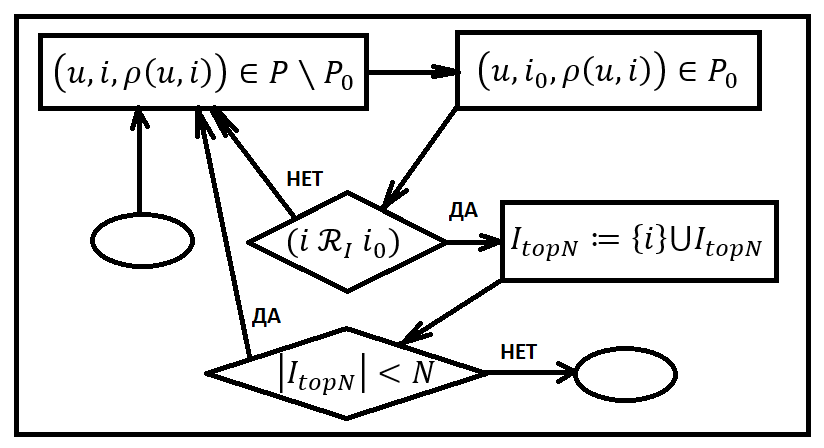
\includegraphics[width=5in,height=3in]{pics/oom_topN.png}
	\end{center}
\end{figure}
Для решения задачи $pred$ необходимо построить множество соседей,
поэтому асимптотическая сложность равна $O(|U|)$ (алгоритм представлен на Рис. 2).
\begin{figure}[H]
	\caption{Алгоритм решения задачи $pred$}
	\begin{center}
		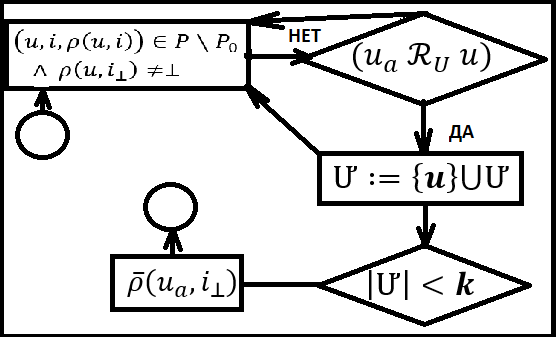
\includegraphics[width=5.5in,height=3in]{pics/prdn-com.png}
	\end{center}
\end{figure}
Реальные системы, к примеру, Amazon, работают с огромным числом пользователей
(свыше 29 миллионов) и объектов (свыше миллиона), поэтому
асимптотическая сложность алгоритмов решений СОМ и ООМ велика в условиях работы
с подобными массивами данных, которые характерны для реальных данных.


{\underline {\bf В третьей главе}} описана разработанная
модель РС, основанная на применении теории нечетких множеств
(далее будем обозначать разработанную модель НРС) и проведено теоретическое
сравнение этой модели с АКМ.\\

Будем представлять контент как нечеткое подмножество множества характеристик и
определим операции объединения и пересечения контентов:
\begin{itemize}
			\item
				$c_X(u) = \{(x | w_U(u, x )) \}, w_U(u, x) \in [0,1]$ ---
				контент пользователя, $x \in X$. При этом множество $X$ не
				обязательно является множеством $I$, как в случае с АКМ, а,
				например, в качестве характеристик может выступать контекстная
				информация.
				$w_U(u, x)$ является
				характеристической функции принадлежности;
			\item
				$c_Y(i) = \{(y | w_I(i, y )) \}, w_I(i, y) \in [0,1]$ ---
				контент объекта, $y \in Y$.
				$w_I(i, x)$ является
				характеристической функции принадлежности;
			\item
				$c_X(u) = \varnothing$, если $w_U(u, x) \equiv 0$ ---
				пустой контент пользователя;
			\item
				$c_Y(i) = \varnothing$, если $w_I(i, y) \equiv 0$ ---
				пустой контент объекта;
			\item
				$c_X(u_1) \bigcup c_X(u_2) = c_X(v): \forall x \in X$ $w_U(v, x) =
				\max(w_U(u_1, x), w_U(u_2, x))$ ---
				объединение контентов пользователей;
			\item
				$c_Y(i_1) \bigcup c_Y(i_2) = c_Y(j): \forall y \in Y$ $w_I(j, y) =
				\max(w_I(i_1, y), w_I(i_2, y))$ ---
				объединение контентов объектов;

			\item
				$c_X(u_1) \bigcap c_X(u_2) = c_X(v): \forall x \in X$ $w_U(v, x) =
				\min(w_U(u_1, x), w_U(u_2, x))$ ---
				пересечение контентов пользователей;
			\item
				$c_Y(i_1) \bigcap c_Y(i_2) = c_Y(j): \forall y \in Y$ $w_I(j, y) =
				\min(w_I(i_1, y), w_I(i_2, y))$ ---
				пересечение контентов объектов.
\end{itemize}

В качестве меры близости объектов будем использовать обобщенное расстояние Хэмминга:
    \begin{equation}
		\label{fuz:rhu}
		\rhu(u,v) =
      \begin{cases}
		  \text{Не определено, если} & c_X(u) \bigcap c_X(v) = \varnothing\\
		  \frac{1}{|X|} \cdot \sum \limits_{x \in X} |w_U(u, x) -
		  w_U(v,x)| & \text{иначе}
      \end{cases}
    \end{equation}

В качестве меры близости пользователей будем использовать обобщенное расстояние Хэмминга:
    \begin{equation}
		\label{fuz:rhi}
		\rhi(i, j) =
      \begin{cases}
         \text{Не определено, если} & c_Y(i) \bigcap
		  c_Y(j) = \varnothing \\
        \frac{1}{|Y|} \cdot \sum \limits_{y \in Y} |w_I(i, y) - w_I(j,y)| & \text{иначе}
      \end{cases}
    \end{equation}
Заданные расстояния обладают метрическими свойствами.

Определим отношение близости пользователей:
\begin{equation}
	\label{fuz:ru}
	u \ru v \Leftrightarrow \rhu(u, v) \le \varepsilon^{\prime}_p :=
	\varepsilon_p.
\end{equation}

Определим отношение близости объектов:
\begin{equation}
	\label{fuz:rt}
i \rt j \Leftrightarrow \rhi(i, j) = \varepsilon_0 := 0.
\end{equation}

Современные РС могут оперировать с контекстной информацией,
а не только информацией о предпочтениях пользователя как
в случае с АКМ.
Этой информацией может быть, к примеру,
социально-демографические данные пользователя или данные о
географическом местоположении.
Разработанная модель позволяет работать
с подобной информацией, поэтому разработанная модель является расширением
АКМ по данным о пользователе. РС производит сопоставление
информации о пользователе и объекте, за счет которого определяется
оценка близости пользователя и объекта. В случае АКМ сопоставление
определяется эвристическими утверждениями.
При работе с более широкой и
неоднозначной информацией о пользователе и при ее сопоставлении с данными об
объектах могут применяться знания эксперта, алгоритмические подходы такие, к примеру,
как машинное обучение и т.д.

В разработанной модели сопоставление информации и пользователе и объекте
определяется заданием
нечеткого отображения $\dc: X \times Y \rightarrow [0,1]$, именуемым оценкой
близости характеристик.

Функция сходства $\dc$ может быть задана в табличной или
аналитической форме алгоритмически или экспертом.

Зададим функцию принадлежности при нечетком отображении $\Psi$ следующим образом:
\begin{equation}
	\label{make-rho1}
		\nu_{\Psi}(y) = \underset{x \in X} {\mathrm{\max}} \min\{
			\delta_c(x,y); w_U(u, x) \}
\end{equation}

С помощью функции $\dc$ можно определить нечеткое отображение $\Psi: X \rightarrow Y$ контента
пользователя на множество контентов объектов.
Для этого
зададим характеристическую функцию принадлежности $\nu_{\Psi}$ характеристики
$y$ нечеткому подмножеству универсального множества $Y$ при отображении $\Psi$ следующей формулой:
\begin{equation}
	\nu_{\Psi}(y) = \underset{x \in X} {\mathrm{\max}} \min\{ \rho(x,y); \mu(x) \}
\end{equation}

Определим функцию отображения контентов пользователей:
\begin{equation}
	\Psi(c_X(u)) = \{ (y | \nu_{\Psi}(y)) \}, y \in Y
\end{equation}

При наличии способа отображения контента пользователя, зададим расстояние
между пользователем $u$ и объектом $i$, значение которого будет выступать в
роли значения прогнозной функции:
	\begin{equation}
		\label{my-rh}
		\rh(u,i) := \rhi(\overline{i}, i)\text{, где }
		c_Y(\overline{i}) := \Psi(c_X(u))
	\end{equation}

\begin{equation}
	\begin{aligned}
	\label{my-pi}
		\text{Нечеткое правило $\Pi_f$ НРС }\\
	\text{заключается в задании оценки сходства } \delta_c\\
	\text{и в дальнейшем расчете прогнозной функции }\rh
	\end{aligned}
\end{equation}

Определим НРС следующим образом:
	\begin{multline}
		(c_X(u) = \{(x | w_U(u, x )) \},\\
		 c_Y(i) = \{(y | w_I(i, y )) \},\\
		\Pi \in \{\Pi_{O}, \Pi_{C}, \Pi_f\}
	\end{multline}
НРС включает правила вывода АКМ,
и поэтому является ее расширением.

{\bf Решения задач в нечеткой модели}.
Определим решения в НРС при использовании $\Pi_f$. Задача $topN$ может быть решена
с помощью линейного поиска объектов, близких к активному пользователю (Рис. 3).
\begin{figure}[H]
	\caption{Алгоритм решения задачи $topN$}
	\begin{center}
		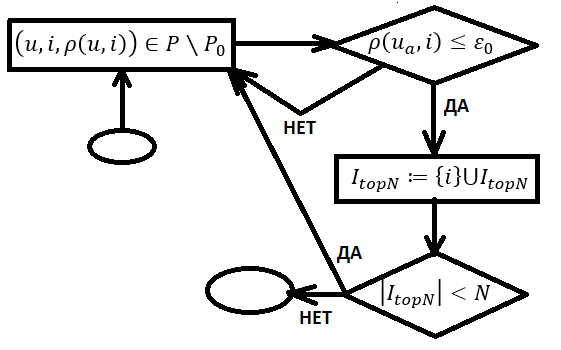
\includegraphics[width=4in,height=2in]{pics/topn-fuz-no-box.png}
	\end{center}
\end{figure}

Задача прогнозирования заключается в вычислении расстояния $\rh(u_a, i_{\bot})$ между
активным пользователем и прогнозируемым объектом.
\begin{figure}[H]
	\caption{Алгоритм решения задачи $topN$}
	\begin{center}
		
\includegraphics[width=3in,height=1in]{pics/prdn-fuz.png}
	\end{center}
\end{figure}

При решении задачи $topN$ максимальное число вычислений $\rh$ равно $n$,
поэтому асимптотическая сложность алгоритма решения равна $O(n)$. Для решения
задачи $pred$ единожды проводится вычисление расстояния,
поэтому асимптотическая сложность алгоритма решения равна $O(1)$.

Проведем сравнение качества НРС и АКМ.

{\bf Сравнение моделей по критерию вычислительной сложности}.
В таблице <<Сравнение асимптотических сложностей>> (\ref{tbl:complex})
приведены асимптотически сложности алгоритмов решений задач в АКМ и НРС.

\begin{table}[h]
	\caption{Сравнение асимптотических сложностей}
	\label{tbl:complex}
  \begin{center}
  \begin{tabular}{|c|c|c|c|}
	\hline
	Модель & Задача & Сложность  \\ \hline
	АКМ & $topN$ & $O(n^2)$  \\ \hline
	АКМ & Прогнозирование & $O(m)$ \\ \hline
	НРС & $topN$ & $O(n)$ \\ \hline
	НРС & Прогнозирование & $O(1)$ \\ \hline
  \end{tabular}
\end{center}
\end{table}
Асимптотические сложности решений задач в НРС
при использовании правила $\Pi_f$ на порядок меньше сложностей
КМ.

{\bf Сравнение моделей по критерию качества решения}.
Рассмотрим качество решений задач по критерию качества
в НРС при использовании $\Pi_O$ и $\Pi_C$.

При решении задачи $pred$ в НРС при применении $\Pi_C$
будем строить кластер соседей следующим образом:
$\mathcal{N}_U = \{ u : \rhu(u_a, u) \le \frac{1}{2} \cdot \varepsilon_p \wedge
(u, i_{\bot}, \rho(u, i_{\bot})) \in P_0)$ \}.
При таком построении кластера выполняется
достаточное условие качественного решения,
что обусловлено
метрическими свойствами используемой в НРС
меры близости $\rhu$ (\ref{fuz:rhu}).

%Покажем, что выполняется достаточное условие. Напомним, что оно
%заключается в выполнении свойства транзитивности отношения близости $\ru$ на
%кластере соседей.
%$\forall u, v \in \mathcal{N}_U$ верно, что
%$(u_a \ru u) \wedge (u_a \ru v)$. Так как функция $\rhu$ обладает
%метрическими свойствами, то $\rhu(u, v) \le \rhu(u_a, u) + \rhu(u_a, v)$.
%По дополнительному условия
%$\rhu(u_a, u) \le \frac{1}{2} \cdot \varepsilon_0$,
%$\rhu(u_a, v) \le \frac{1}{2} \cdot \varepsilon_0$,
%поэтому $\rhu(u, v) \le \varepsilon_p \Rightarrow u \ru v$.

При решении задачи $topN$ в НРС при применении $\Pi_O$
выполняется достаточное условие качественного решения,
что обусловлено заданием отношения $\rt$ (\ref{fuz:rt})
в НРС и метрическими свойствами используемой в
НРС меры близости $\rhi$ (\ref{fuz:rhi}).

Так как в НРС при использовании $\Pi_C$ и $\Pi_O$
выполняются достаточные условия качественных решений, то
разработанная модель является качественной модификацией АКМ.

Эффективность НРС по критерию качества при применении правила
вывода $\Pi_f$ так же, как и в АКМ ограничена
дополнительным условием.
В обеих моделях выполнение условий
зависит от разработчика: для АКМ это выбор функции $\rhi, \rhu$ и порогового
значения $\varepsilon_i, \varepsilon_u$, для НРС --- это
определение $\delta_c$.
Однако при работе с АКМ
разработчик обладает меньшей свободой действий, чем при работе с
НРС, так как он может варьировать только функцию, которая будет
использоваться в качестве меры близости, и ее пороговое значение.
При работе с НРС разработчик может варьировать
алгоритмы, эвристики, наборы данных, знания
экспертов и т.п., чтобы задать $\delta_c$ и зависящее от этой функции $\Pi_f$.

{\bf Вывод}: разработана математическая модель РС, которая теоретически
более качественна, чем АКМ, и является ее расширением.


{\underline {\bf В четвертой главе}} описано программное обеспечение, которое
было использовано для проведения тестировании, приведены результаты
тестирования, на основании которых проведено практическое сравнение АКМ
и разработанной модели.

Тесты проводились на новейшем множестве данных MovieLens Small.
Эти исходные данные были собраны компанией MovieLens, которая
занимается исследованиями и разработками в области РС. Исходные
данные являются данными,
которые были заполнены реальными
пользователями. Характеристики используемого множества данных:
\begin{itemize}
	\item $|U| = 700$;
	\item $|I| = 9000$ --- объектами являются фильмы
	\item $|P| = 100 000$ --- значениями $\rho(u, i)$ являются оценки
		пользователей, которые были ими заданы в соответствии со своим
		предпочтением к конкретному фильму;
	\item $|Y|$ --- характеристиками объектов являются кинематографические
		жанры;
	\item $X = I$ --- характеристиками пользователей для АКМ являются объекты.
\end{itemize}

Для АКМ $X = I$ и $w_U(u, x) = \rho(u,x), x \in I$.

Для задания правила вывода $\Pi_f$ была аналитически определена
функция $\delta_c$, основываясь на эвристическом предположении о том,
что между оценкой близости $\rho(u, i)$, заданной пользователем $u$
и характеристикой $y \in Y$ объекта $i$,
то есть жанром фильма, существует корреляция:
\begin{multline}
	\delta_c(i, y) = \frac{1}{|\{i: \exists \rho(u,i)\}|}
	\cdot
	|\{ i : (\rho(u, i) < \varepsilon_1) \wedge (\nu(y) = 1)\}| -\\
	|\{ i : (\rho(u, i) > \varepsilon_2) \wedge (\nu(y) = 1)\}|, \\
	\text{ где }
	\varepsilon_1 = 0,2, \varepsilon_2 = 0,6;
\end{multline}

Такое эвристическое предположение верно не для всех пользователей, так как
их вкусы могут быть неоднородными. Поэтому для некоторых пользователей функция
$\delta_c$ задана так, что
$|\rh(u, i_{\bot}) - \rho(u, i_{\bot}) \le \varepsilon_p|$,
а для некоторых --- нет.

Для проведения тестов исходные данные были
стандартно разбиты на тестовое и обучающее множество по следующему принципу:
разбиение проводилось случайно, в обучающее множество входит
80\% данных, в тестовое --- оставшиеся 20\%.

{\bf Сравнение моделей по критерию вычислительной сложности} \\
В качестве показателя вычислительной сложности алгоритма рассмотрим время,
которое затрачивается в среднем на решение задачи для одного пользователя.
Решение задачи $topN$ рассмотрим для $N = 10$, решение задачи $pred$
для одного прогнозируемого объекта. Алгоритмы использовались те же, что
применялись при определении качества решения, описанные выше.
Для оценки качества решения задачи $topN$ использовалась функция $1 -
\text{точность}$, для решения задачи $pred$ --- $NMAE$.

Тесты проводились на следующем оборудовании:
\begin{itemize}
	\item ОС --- Ubuntu 16.04 LS, 64 бита;
	\item Оперативная память --- 8Gb;
	\item Процессор --- Intel Core i5-4460 CPU @ 3.20GHz $\times$ 4;
\end{itemize}

\begin{table}[htb]
	\caption{Время решения задачи $topN$}
  \begin{center}
	\label{table:time-topn}
	\begin{tabular}{|c|c|}
	  \hline
		Модель & Время (с)\\ \hline
		ООМ& 13\\ \hline
		НРС&0,06 \\ \hline
	\end{tabular}
  \end{center}
\end{table}
%Столь длительное по времени решение задачи $topN$
%объясняется тем, что для решения этой задачи ведется работа
%с матрицей $\mathcal{M}$, в которой хранятся значения
%$\di$, по алгоритму приходится делать $|I|$ запросов к базе, по которому
%достается $|I|$ значений. Хранить целиком в памяти матрицу не оптимально по
%отношению к расходуемой оперативной памяти, а для реальных систем и вовсе может
%быть невозможно, где мощность множества объектов велика. Конечно,
%каждый шаг алгоритма можно оптимизировать и задействовать методы, ускоряющие
%работу алгоритма, однако целью исследования было сравнить стандартные
%предлагаемые подходы, а не оптимизировать по времени существующие.

\begin{table}[htb]
\caption{Время решения задачи $pred$}
  \begin{center}
	\label{table:time-p}
	\begin{tabular}{|c|c|}
	  \hline
		Модель & Время (с)\\ \hline
		СОМ& 0,5\\ \hline
		НРС&0,08 \\ \hline
	\end{tabular}
  \end{center}
\end{table}

В НРС определены алгоритмы, которые заметно эффективней
по критерию вычислительной сложности.
Практические результаты подтверждают вывод о том, что НРС является
эффективным расширением АКМ по критерию вычислительной сложности.

{\bf Влияние свойства транзитивности на ООМ при решении задачи $topN$} \\
Задача $topN$ решалась в ООМ при применении меры сходства единица минус косинус в качестве
$\rhi$ и $\varepsilon_i \in \{0,49; 0,1\}$.
При $\varepsilon_i = 0,1$ вероятность того, что $(i \rt j) \wedge (j \rt k)
\Rightarrow (i \rt k)$, выше, чем при $\varepsilon_i = 0,49$.
На Рис. \ref{pic:topn_trans} приведены результаты решений задачи $topN$ при
различных пороговых значениях. Черным цветом приведены результаты для
$\varepsilon_i = 0,1$, красным --- для $\varepsilon_i = 0,49$.
Видно, что при $\varepsilon_i = 0,1$ результаты решений эффективней.

Некоторые результаты при $\varepsilon_i = 0,1$ хуже, чем при
$\varepsilon_i = 0,49$. Это происходит для тех пользователей,
для которых характерно свойство неоднородности.

\begin{figure}[H]
	\caption{Влияние свойства транзитивности на ООМ при решении задачи $topN$}
	\label{pic:topn_trans}
	\begin{center}
		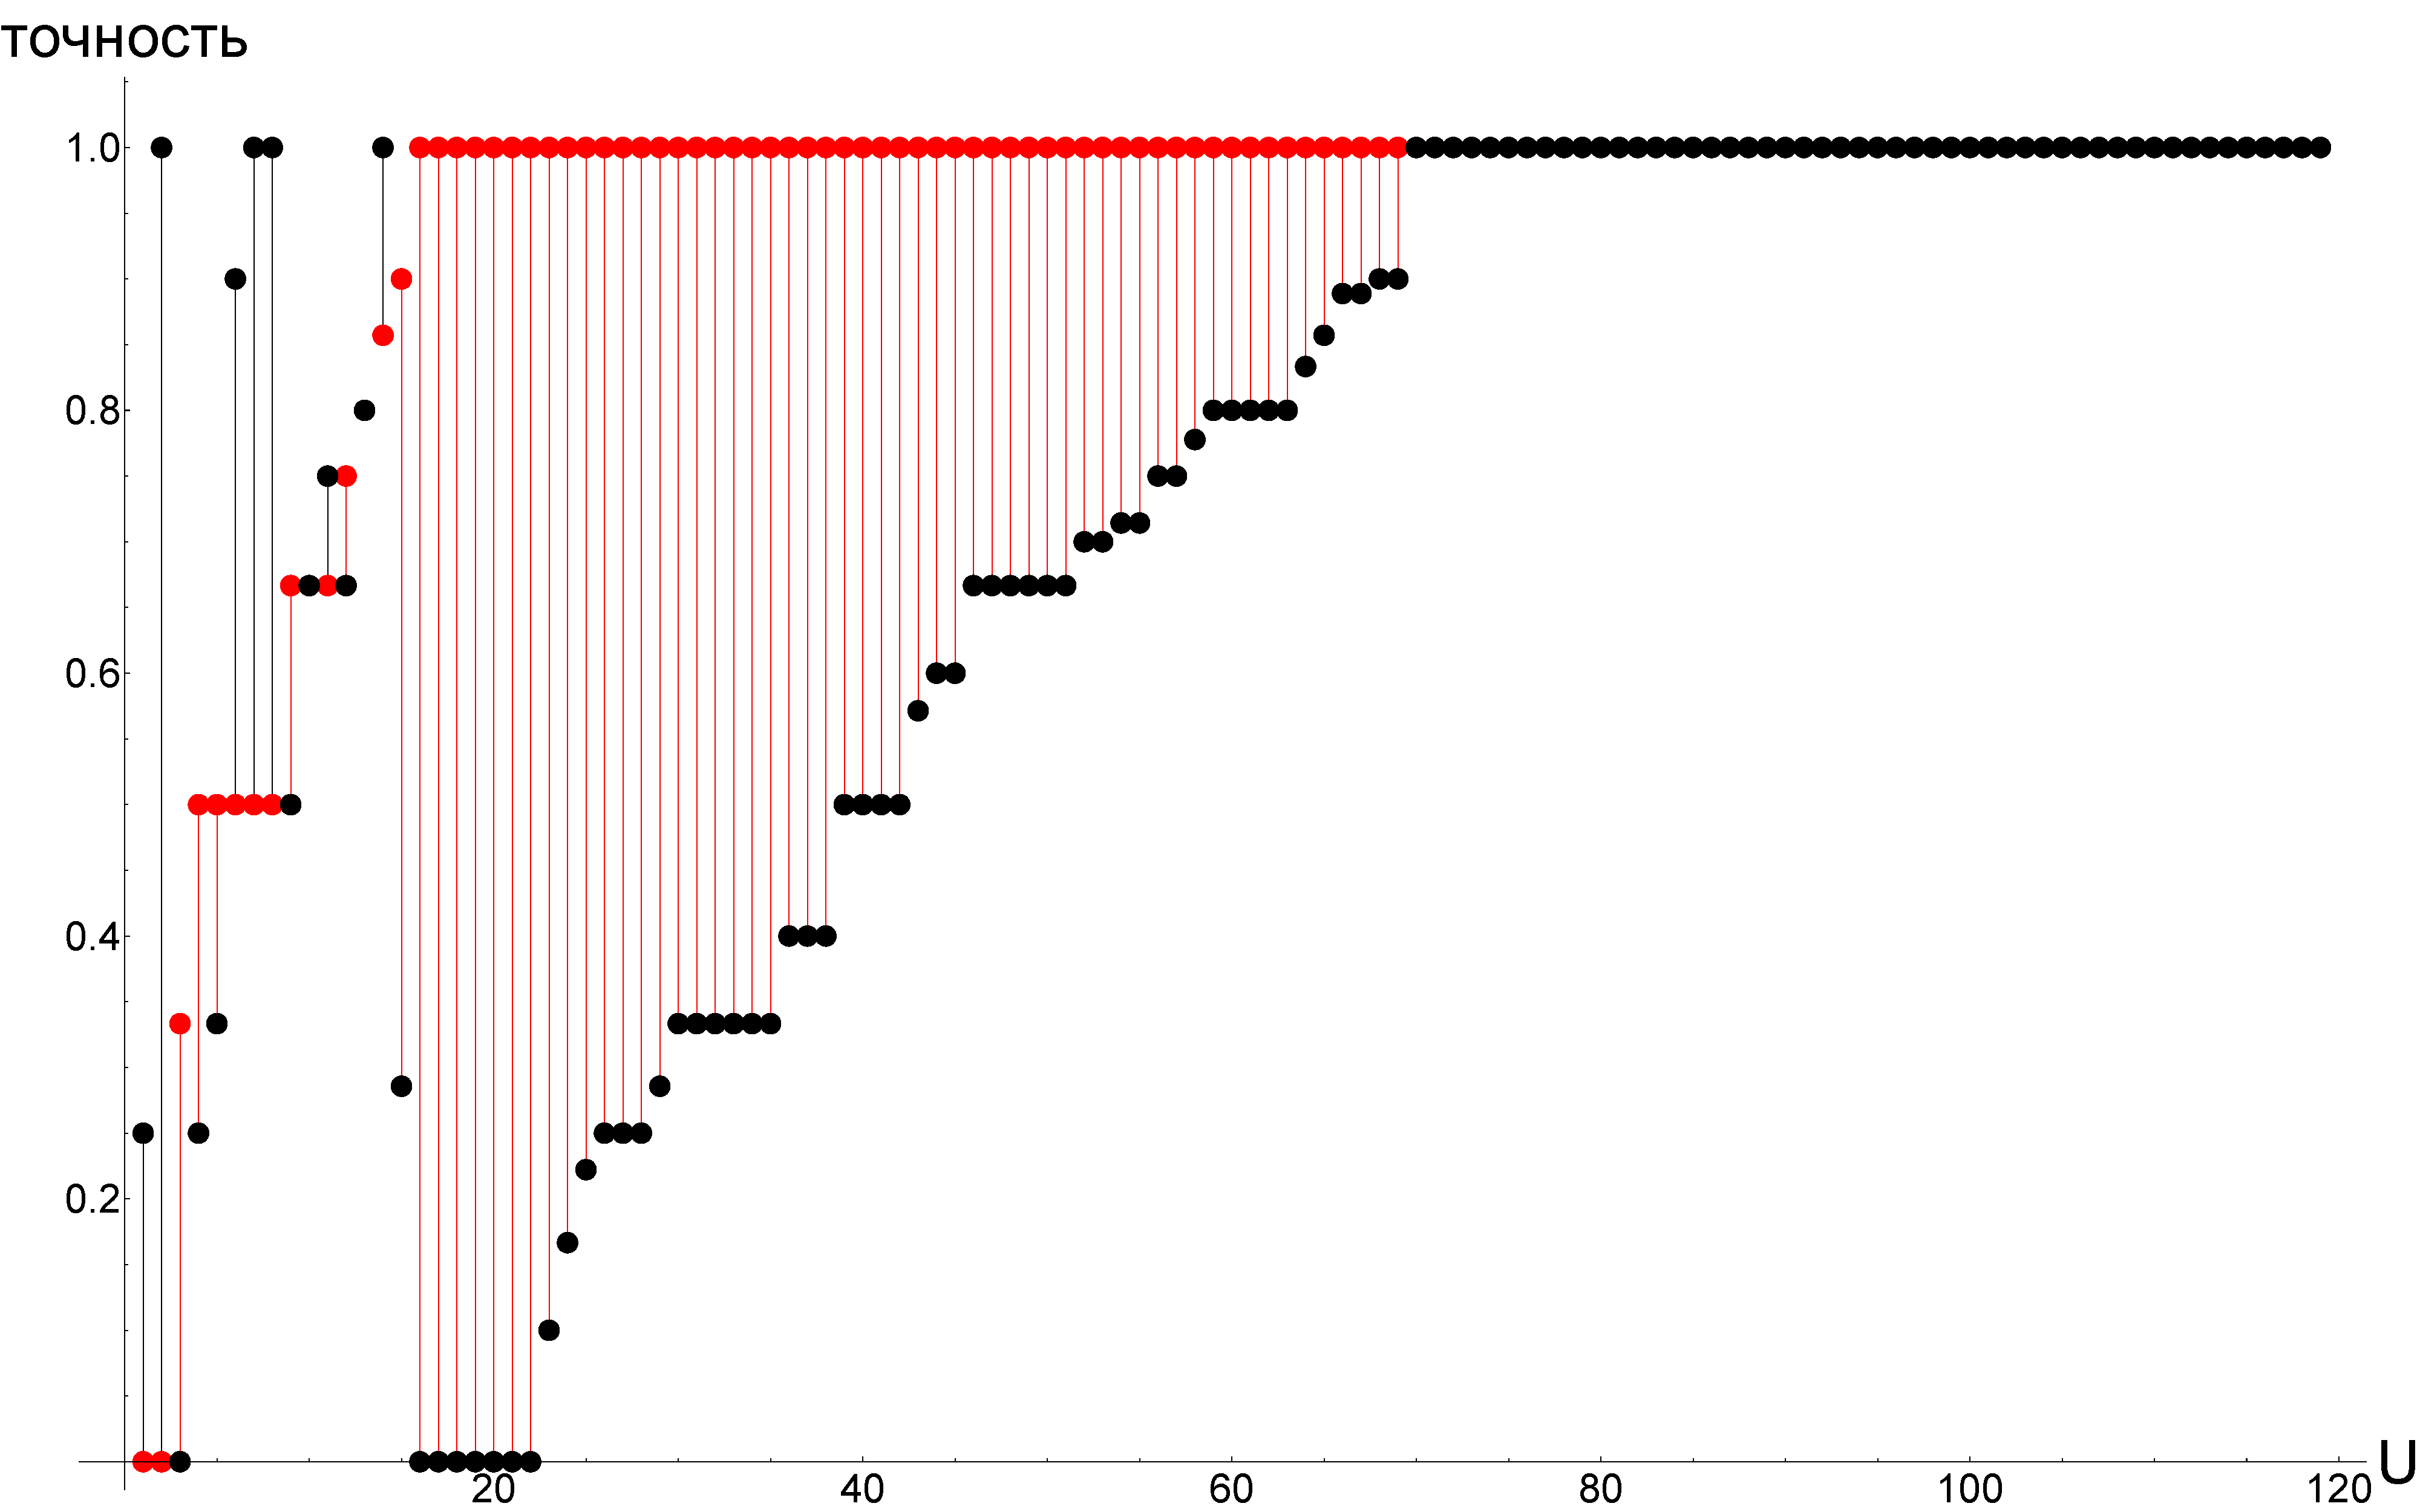
\includegraphics[width=5in,height=2in]{pics/results/transitivity.pdf}
\end{center}
\end{figure}

{\bf Влияние свойства транзитивности на СОМ при решении задачи $pred$} \\
Задача $pred$ была решена в РОМ при применении меры сходства
единица минус коэффициент корреляции Пирсона в качестве $\rhu$ и
$\varepsilon_p = \{0,49; 0,1\}$.
При $\varepsilon_p = 0,1$ вероятность того, что $(i \ru j) \wedge (j \ru k)
\Rightarrow (i \ru k)$, выше, чем при $\varepsilon_p = 0,49$.
На Рис. \ref{pic:pred_trans} приведены результаты решений задачи $pred$ при
различных пороговых значениях. Черным цветом приведены результаты для
$\varepsilon_p = 0,1$, красным --- для $\varepsilon_p = 0,49$.
Видно, что при $\varepsilon_p = 0,1$ результаты решений эффективней.

\begin{figure}[H]
	\caption{Влияние свойства транзитивности на СОМ при решении задачи $pred$}
	\label{pic:pred_trans}
	\begin{center}
		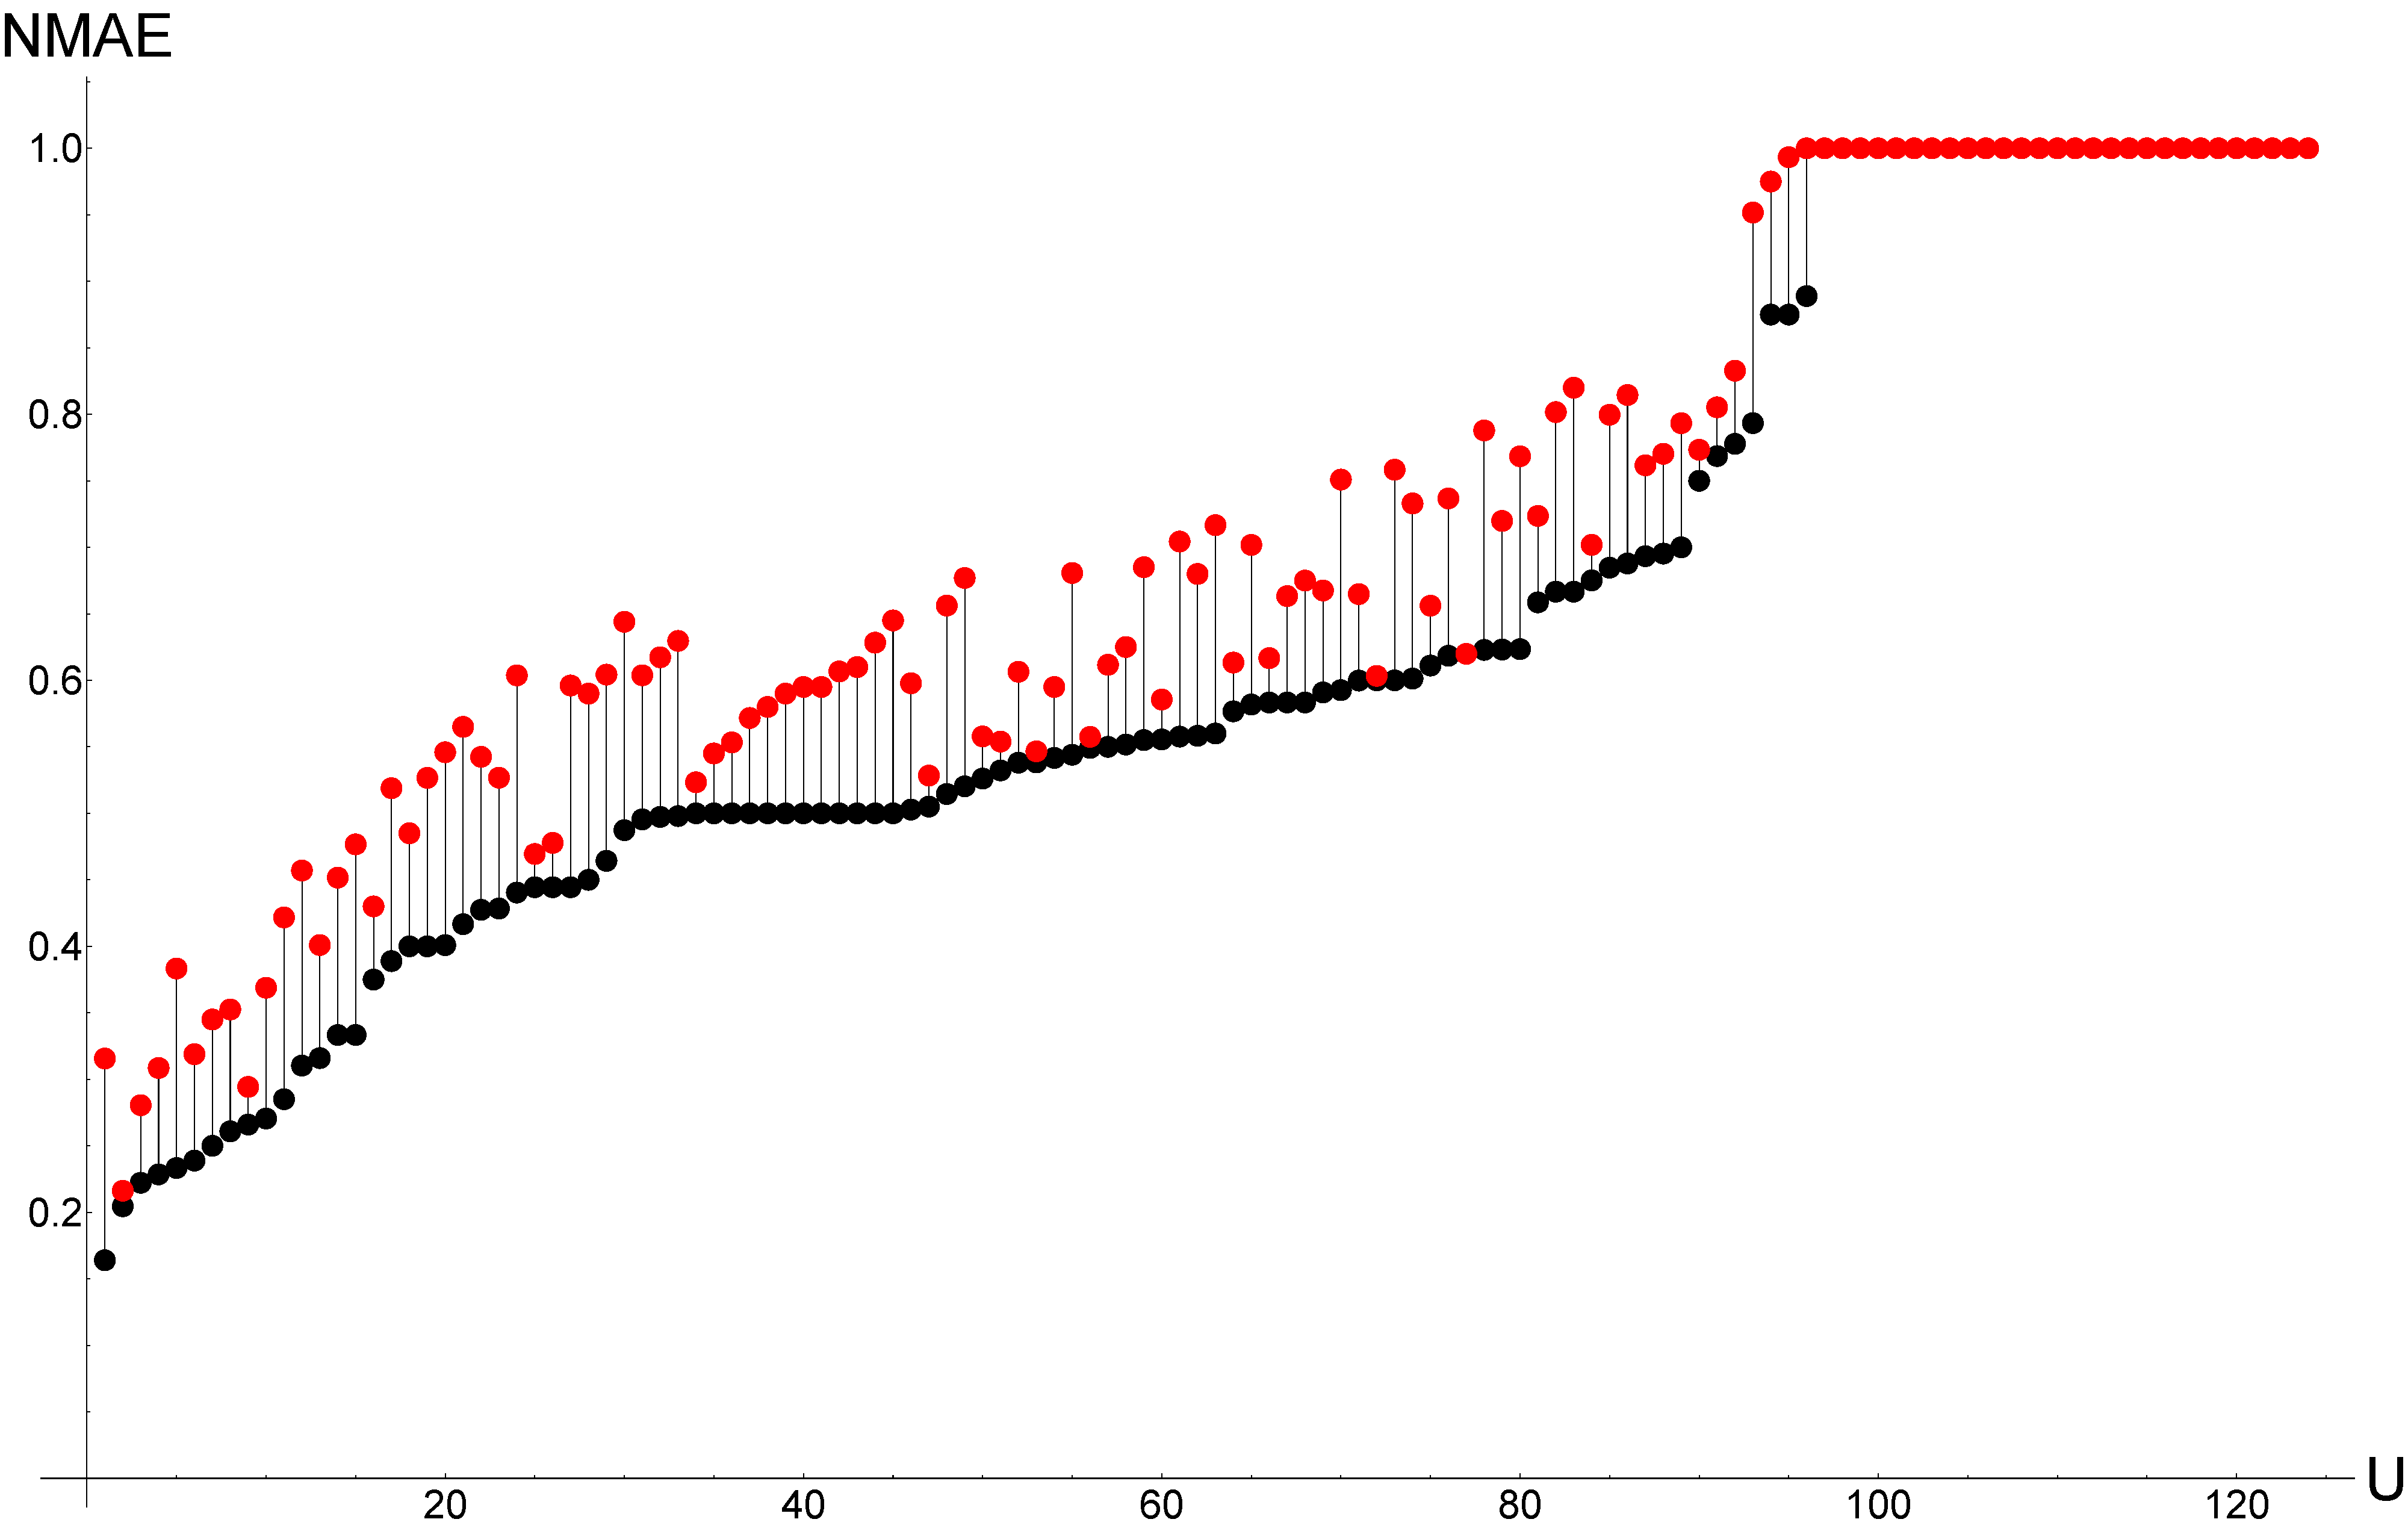
\includegraphics[width=5in,height=2in]{pics/results/ub_transitivity.pdf}
\end{center}
\end{figure}

%TODO: для задачи топн объяснить так, почему иногда хуже при применении
% п_о: в силу свойства неоднородности. На самом деле это говорит о том,
% что модель работает хорошо

%TODO: Написать, что оценки качества коррелируют меж собой, поэтому используем
%один показатель
{\bf Качество решений задачи $topN$ к при использовании $\Pi_O$ в НРС и ООМ}\\
На Рис. \ref{pic:topn_pio} приведены результаты решения
задачи $topN$ при применении $\Pi_O$ в ООМ и НРС.
Черным цветом обозначены результаты решения в НРС.
Видно, что в большинстве НРС более эффективна по критерию качества,
в других ситуациях предпочтения пользователя неоднородны.

\begin{figure}[H]
	\caption{Качество решений задачи $topN$ при использовании $\Pi_O$ в ООМ и
	НРС}
	\label{pic:topn_pio}
	\begin{center}
		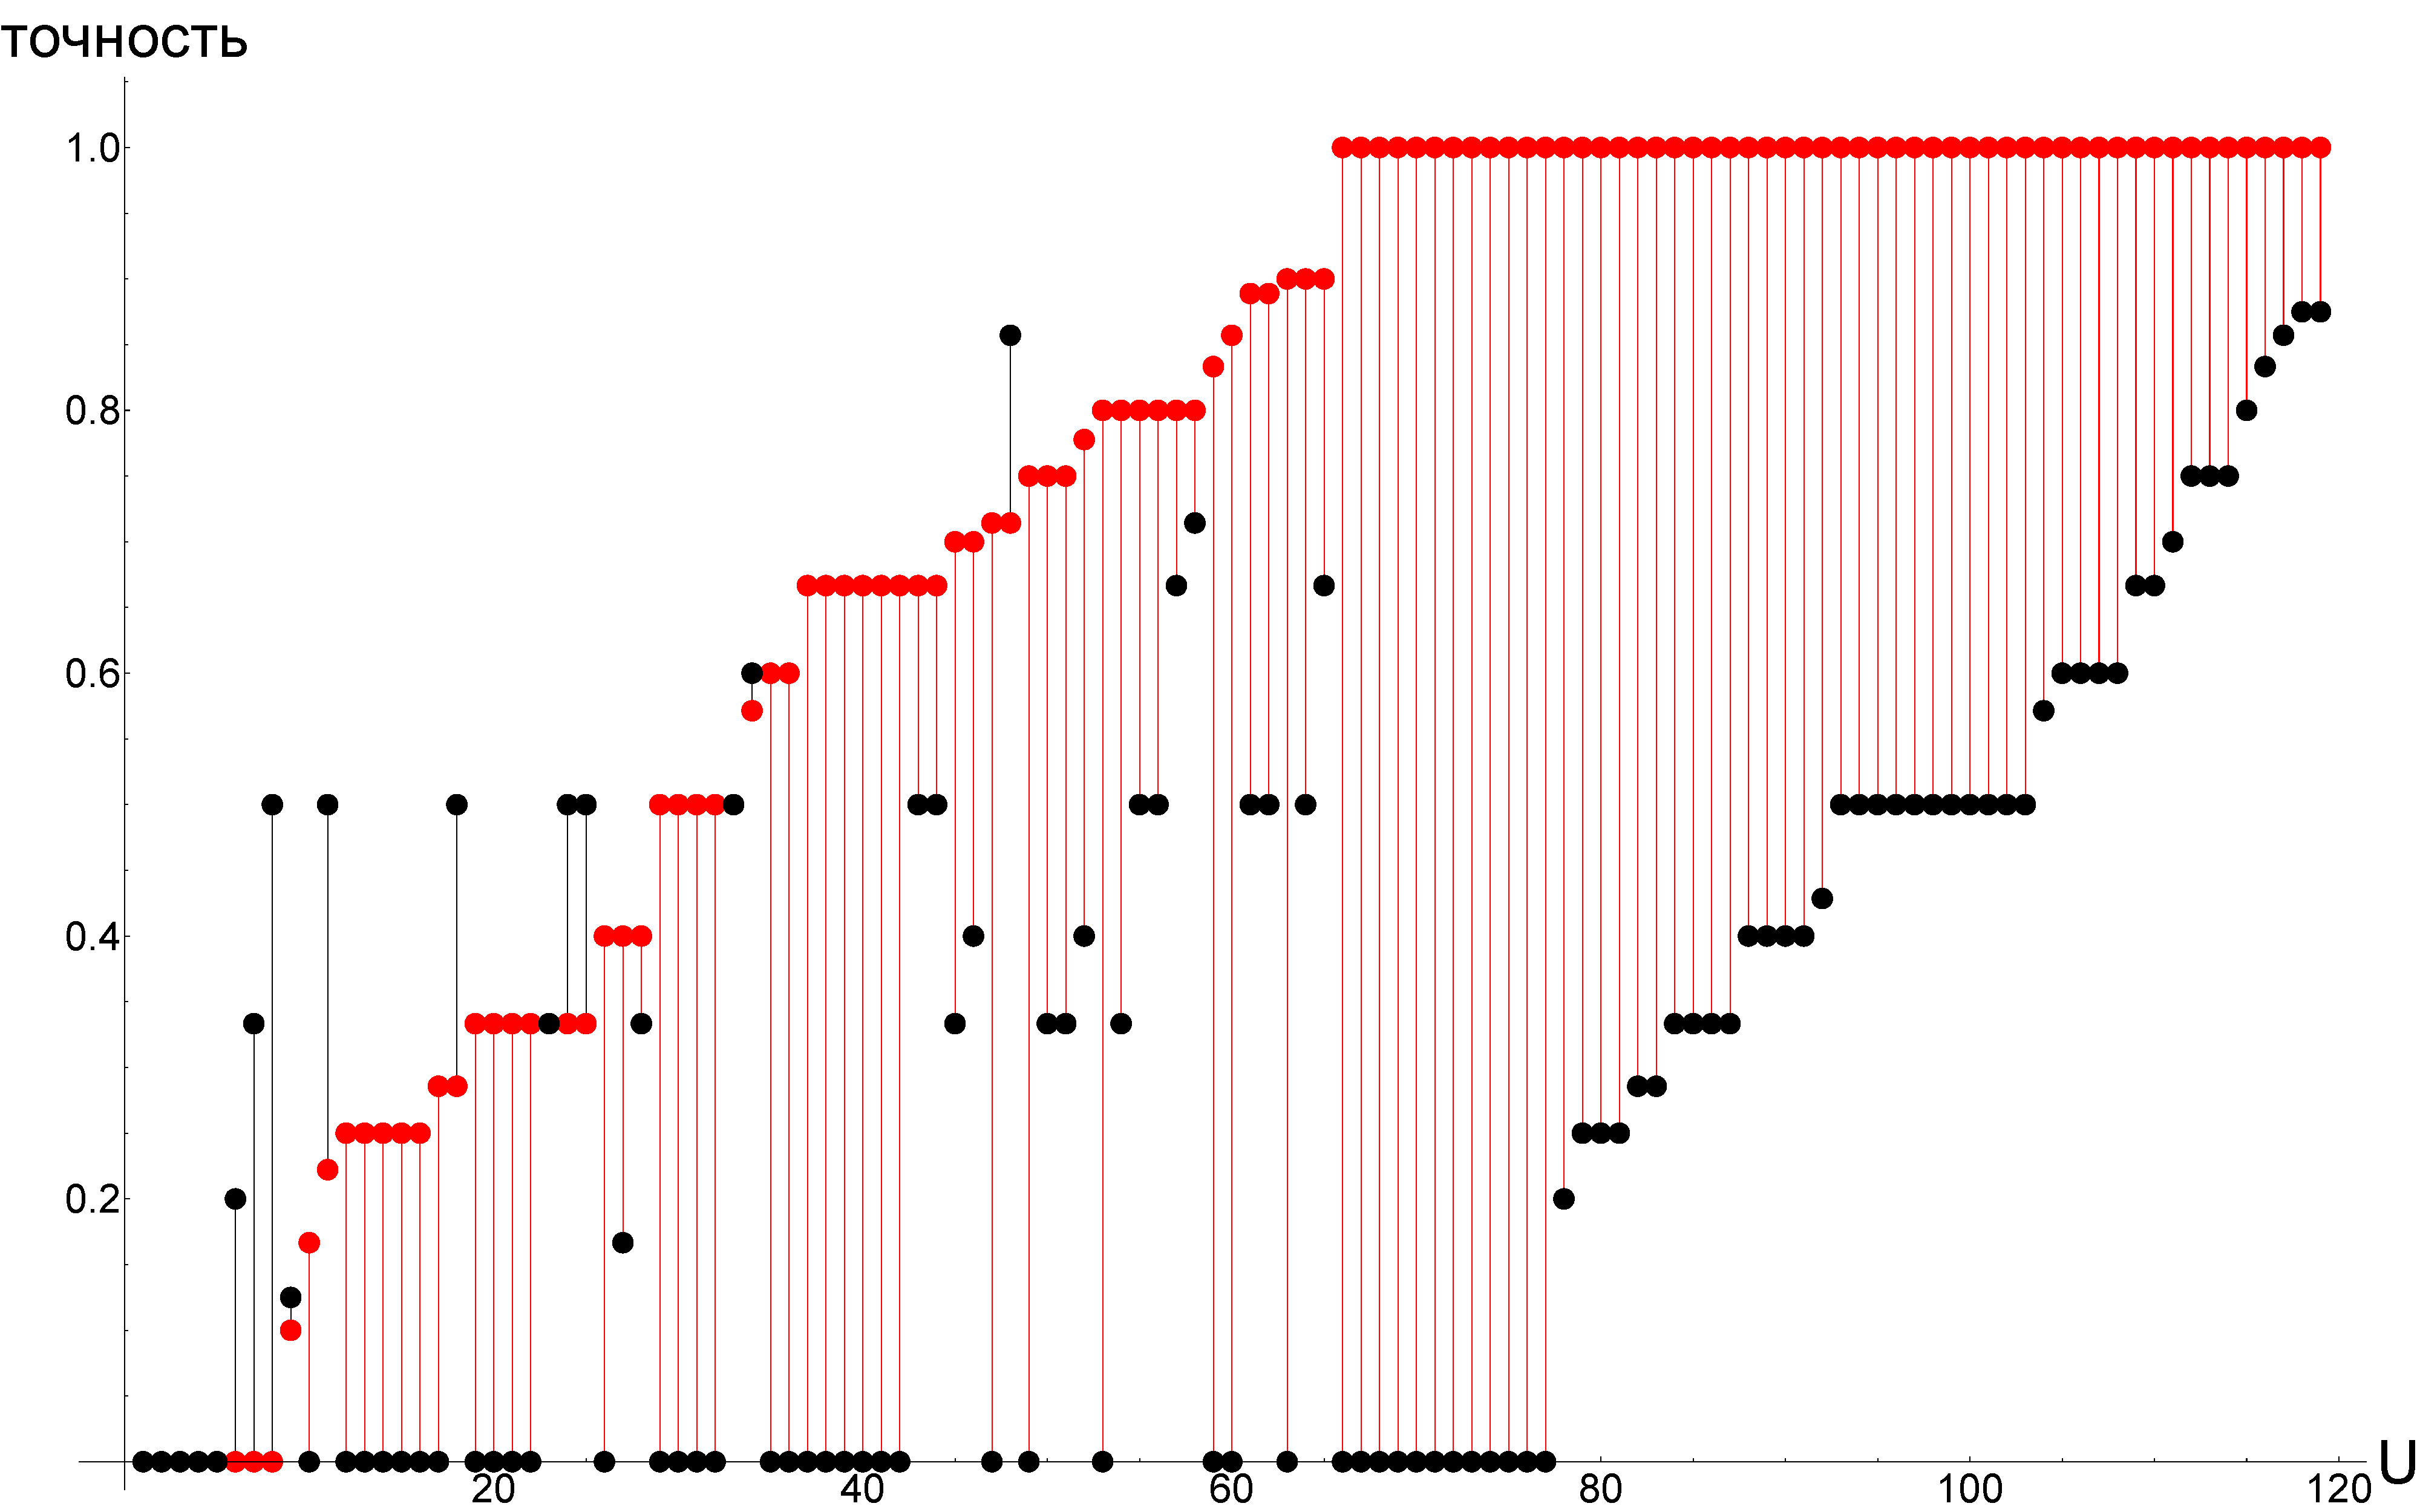
\includegraphics[width=5in,height=2in]{pics/results/ib_method_in_ib_and_fuzzy_model.pdf}
\end{center}
\end{figure}

{\bf Качество решений задачи $topN$ при использовании $\Pi_O$ в ООМ и $\Pi_f$ в
НРС}\\
На Рис. \ref{pic:topn_pio_pif} приведены результаты решения
задачи $topN$ при применении $\Pi_O$ в ООМ и $\Pi_f$ в НРС.
Черным цветом обозначены результаты решения в НРС.
Видно, что НРС более эффективна по критерию качества.

\begin{figure}[H]
	\caption{Качество решений задачи $topN$ при использовании $\Pi_O$ в ООМ и
	$\Pi_f$ в НРС}
	\label{pic:topn_pio_pif}
	\begin{center}
		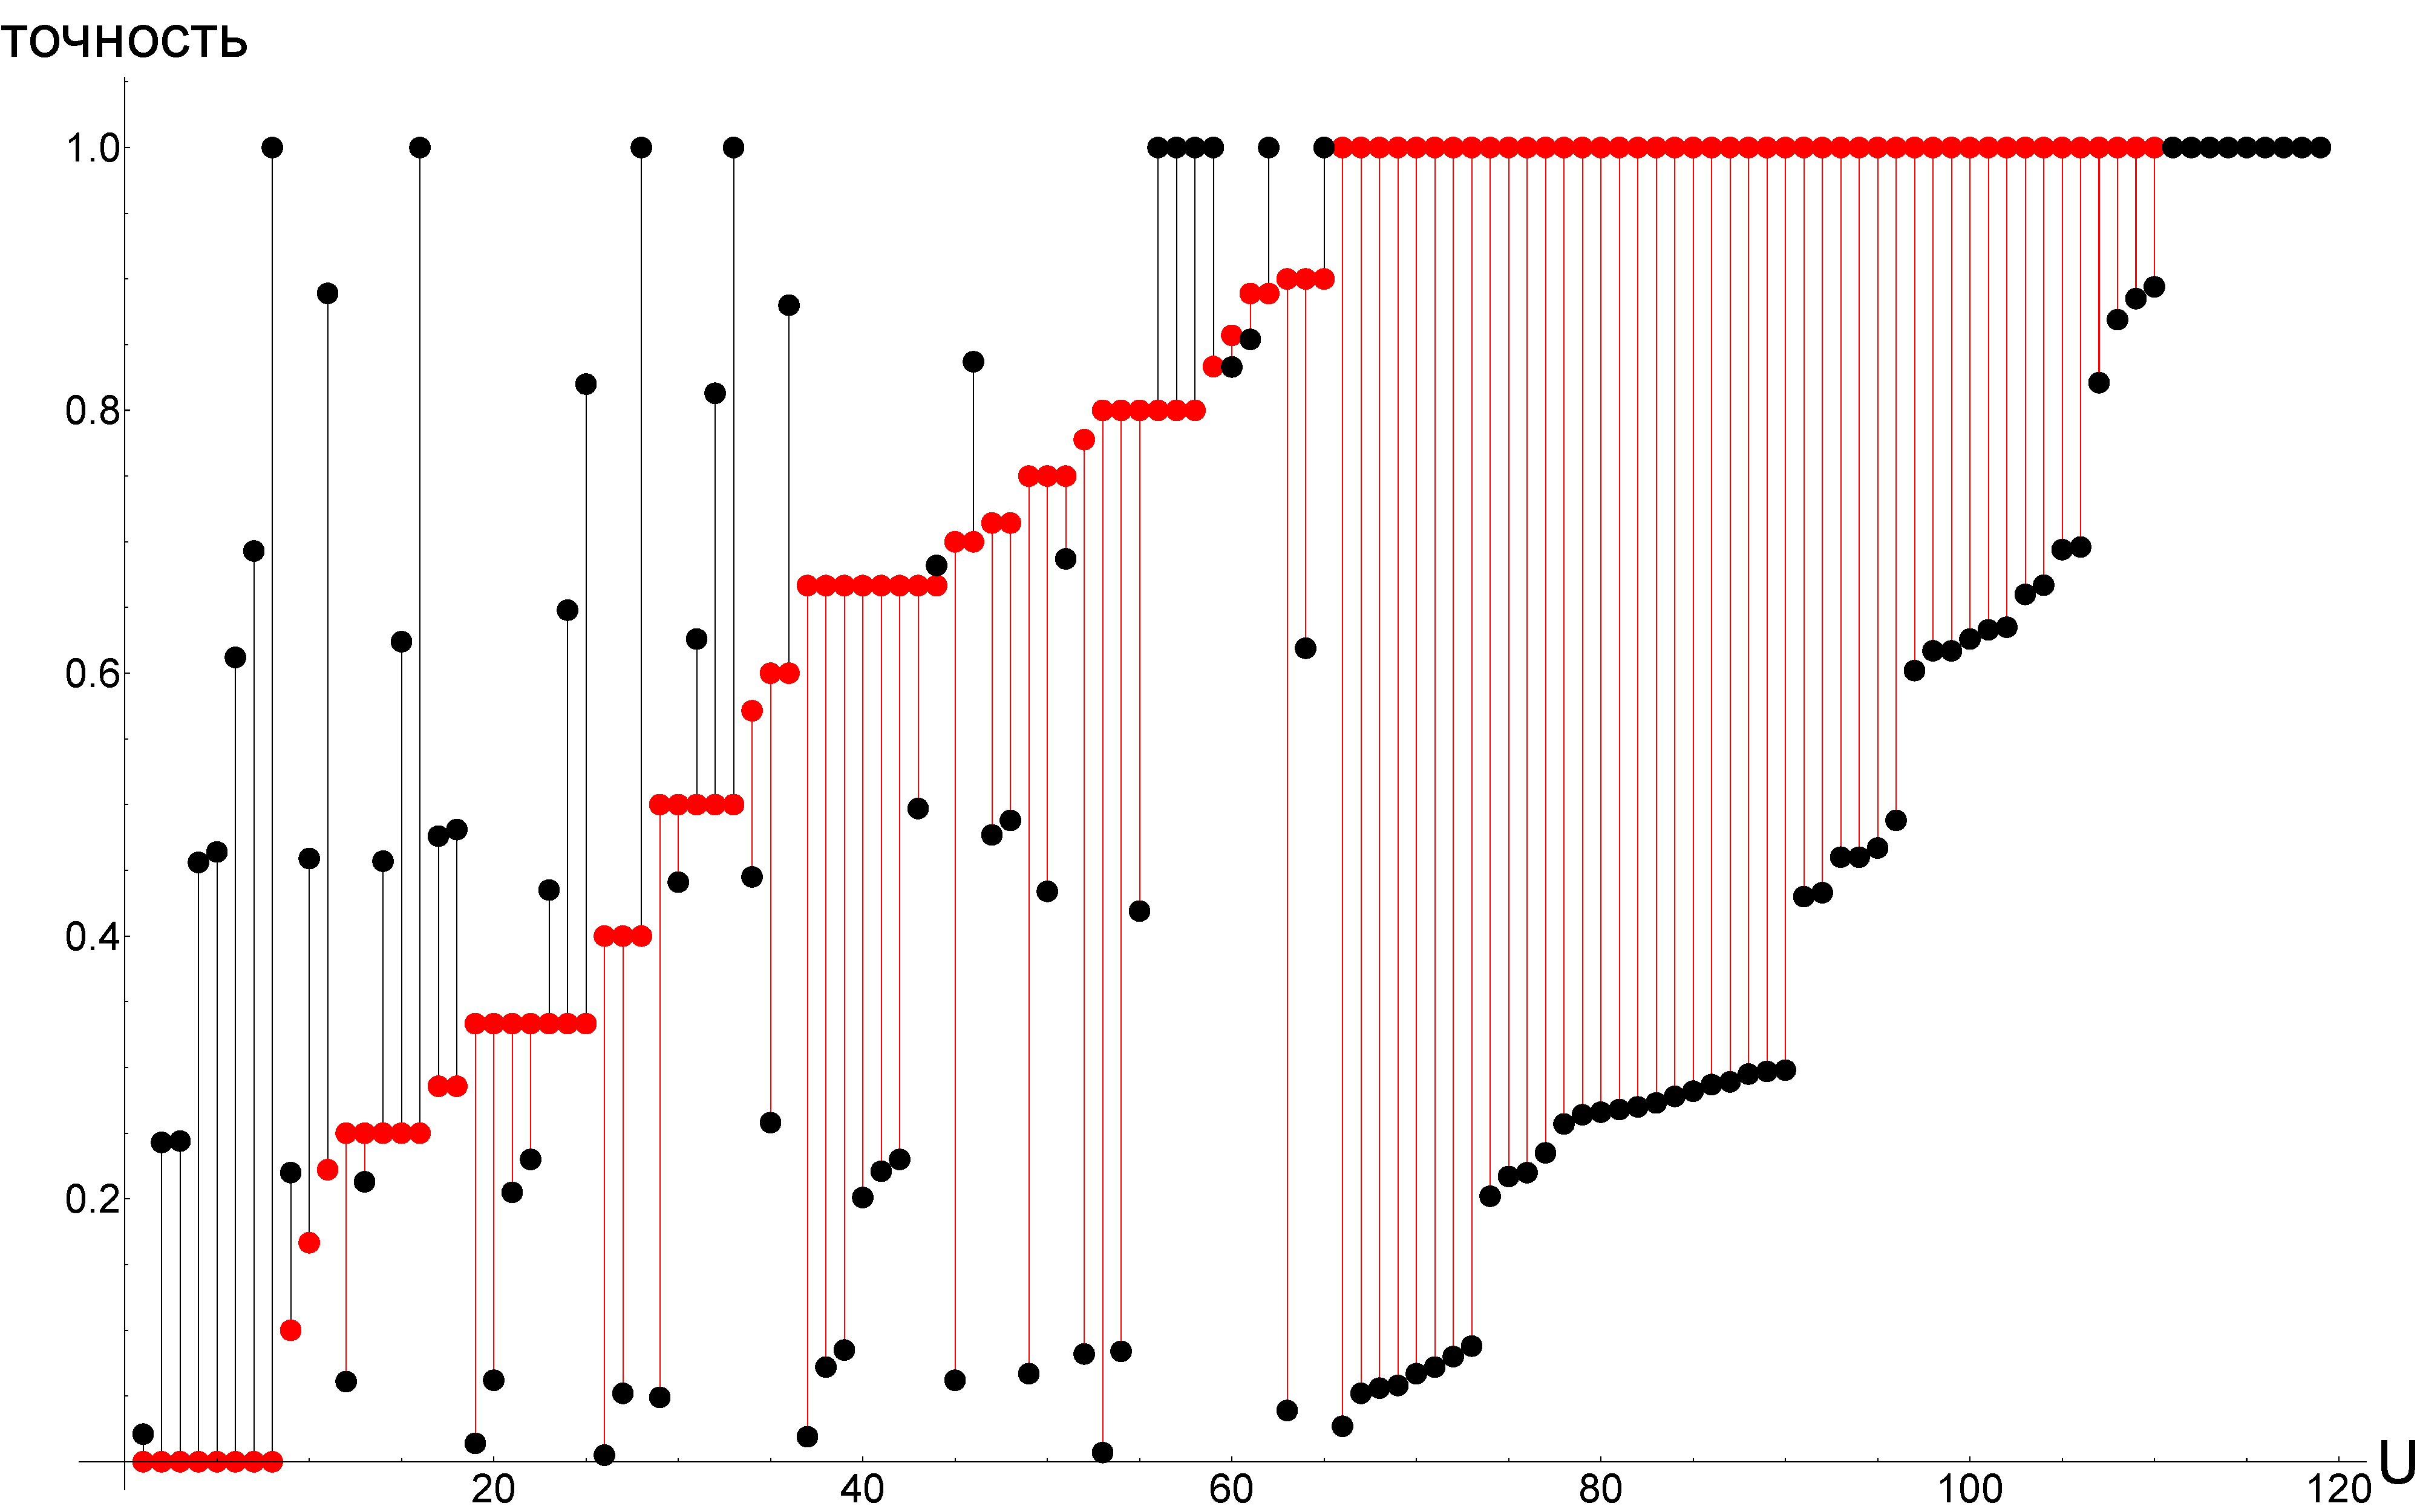
\includegraphics[width=5in,height=2in]{pics/results/topn_oom_fuzz.pdf}
\end{center}
\end{figure}
Видно, что в большинстве НРС более эффективна по критерию качества,
в других ситуациях предпочтения пользователя неоднородны,
и эвристическое предположение, на котором основано построение
функции $\delta_c$, не верно для пользователя.


{\bf Качество решений задачи $pred$ к при использовании $\Pi_C$ в СОМ и НРС}
На Рис. \ref{pic:pred_pic} приведены результаты решения
задачи $pred$ при применении $\Pi_C$ в СОМ и НРС.
Черным цветом обозначены результаты решения в НРС.

\begin{figure}[H]
	\caption{Качество решений задачи $pred$ при использовании $\Pi_C$ в СОМ и
	НРС}
	\label{pic:pred_pic}
	\begin{center}
		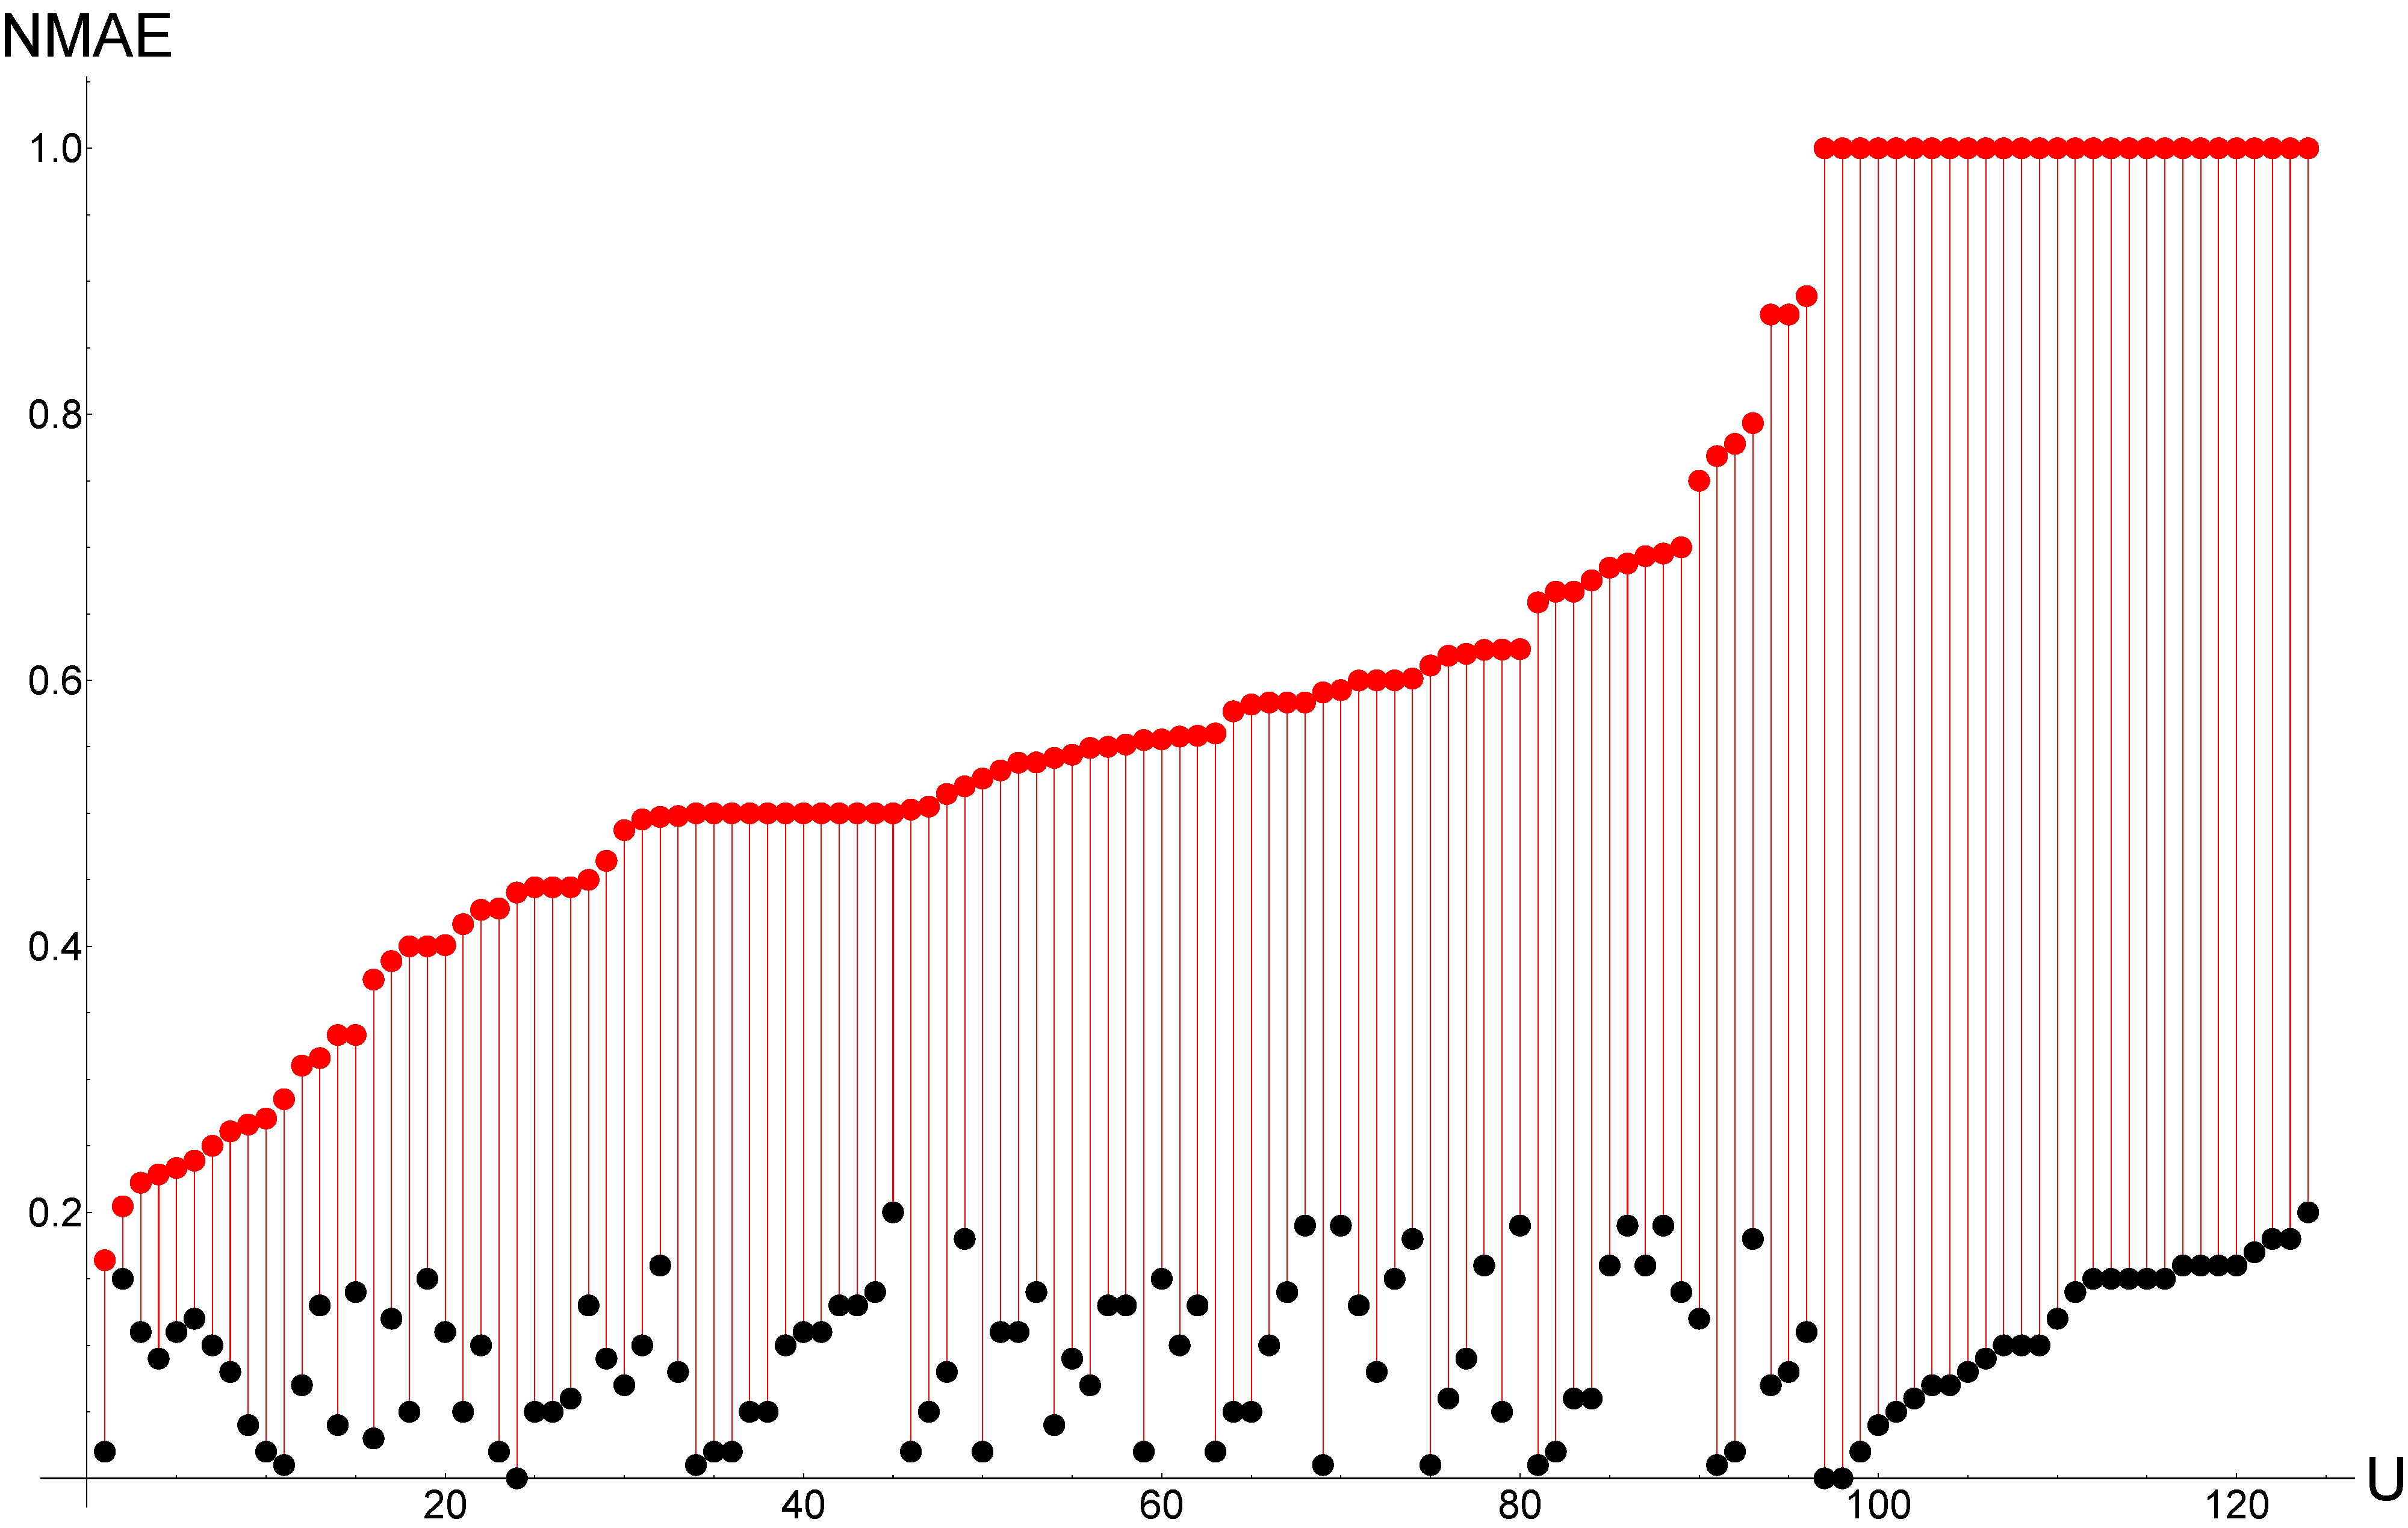
\includegraphics[width=5in,height=2in]{pics/results/ub_method_in_ub_and_fuzz_model.pdf}
\end{center}
\end{figure}
Видно, что в большинстве НРС более эффективна по критерию качества,
в других ситуациях предпочтения пользователя неоднородны.

{\bf Качество решений задачи $pred$ при использовании $\Pi_C$ и $\Pi_f$}
На Рис. \ref{pic:pred_pio_pif} приведены результаты решения
задачи $pred$ при применении $\Pi_C$ в СОМ и $\Pi_f$ в НРС.
Черным цветом обозначены результаты решения в НРС.

\begin{figure}[H]
	\caption{Качество решений задачи $pred$ при использовании $\Pi_C$ в СОМ и
	$\Pi_f$ в НРС}
	\label{pic:pred_pio_pif}
	\begin{center}
		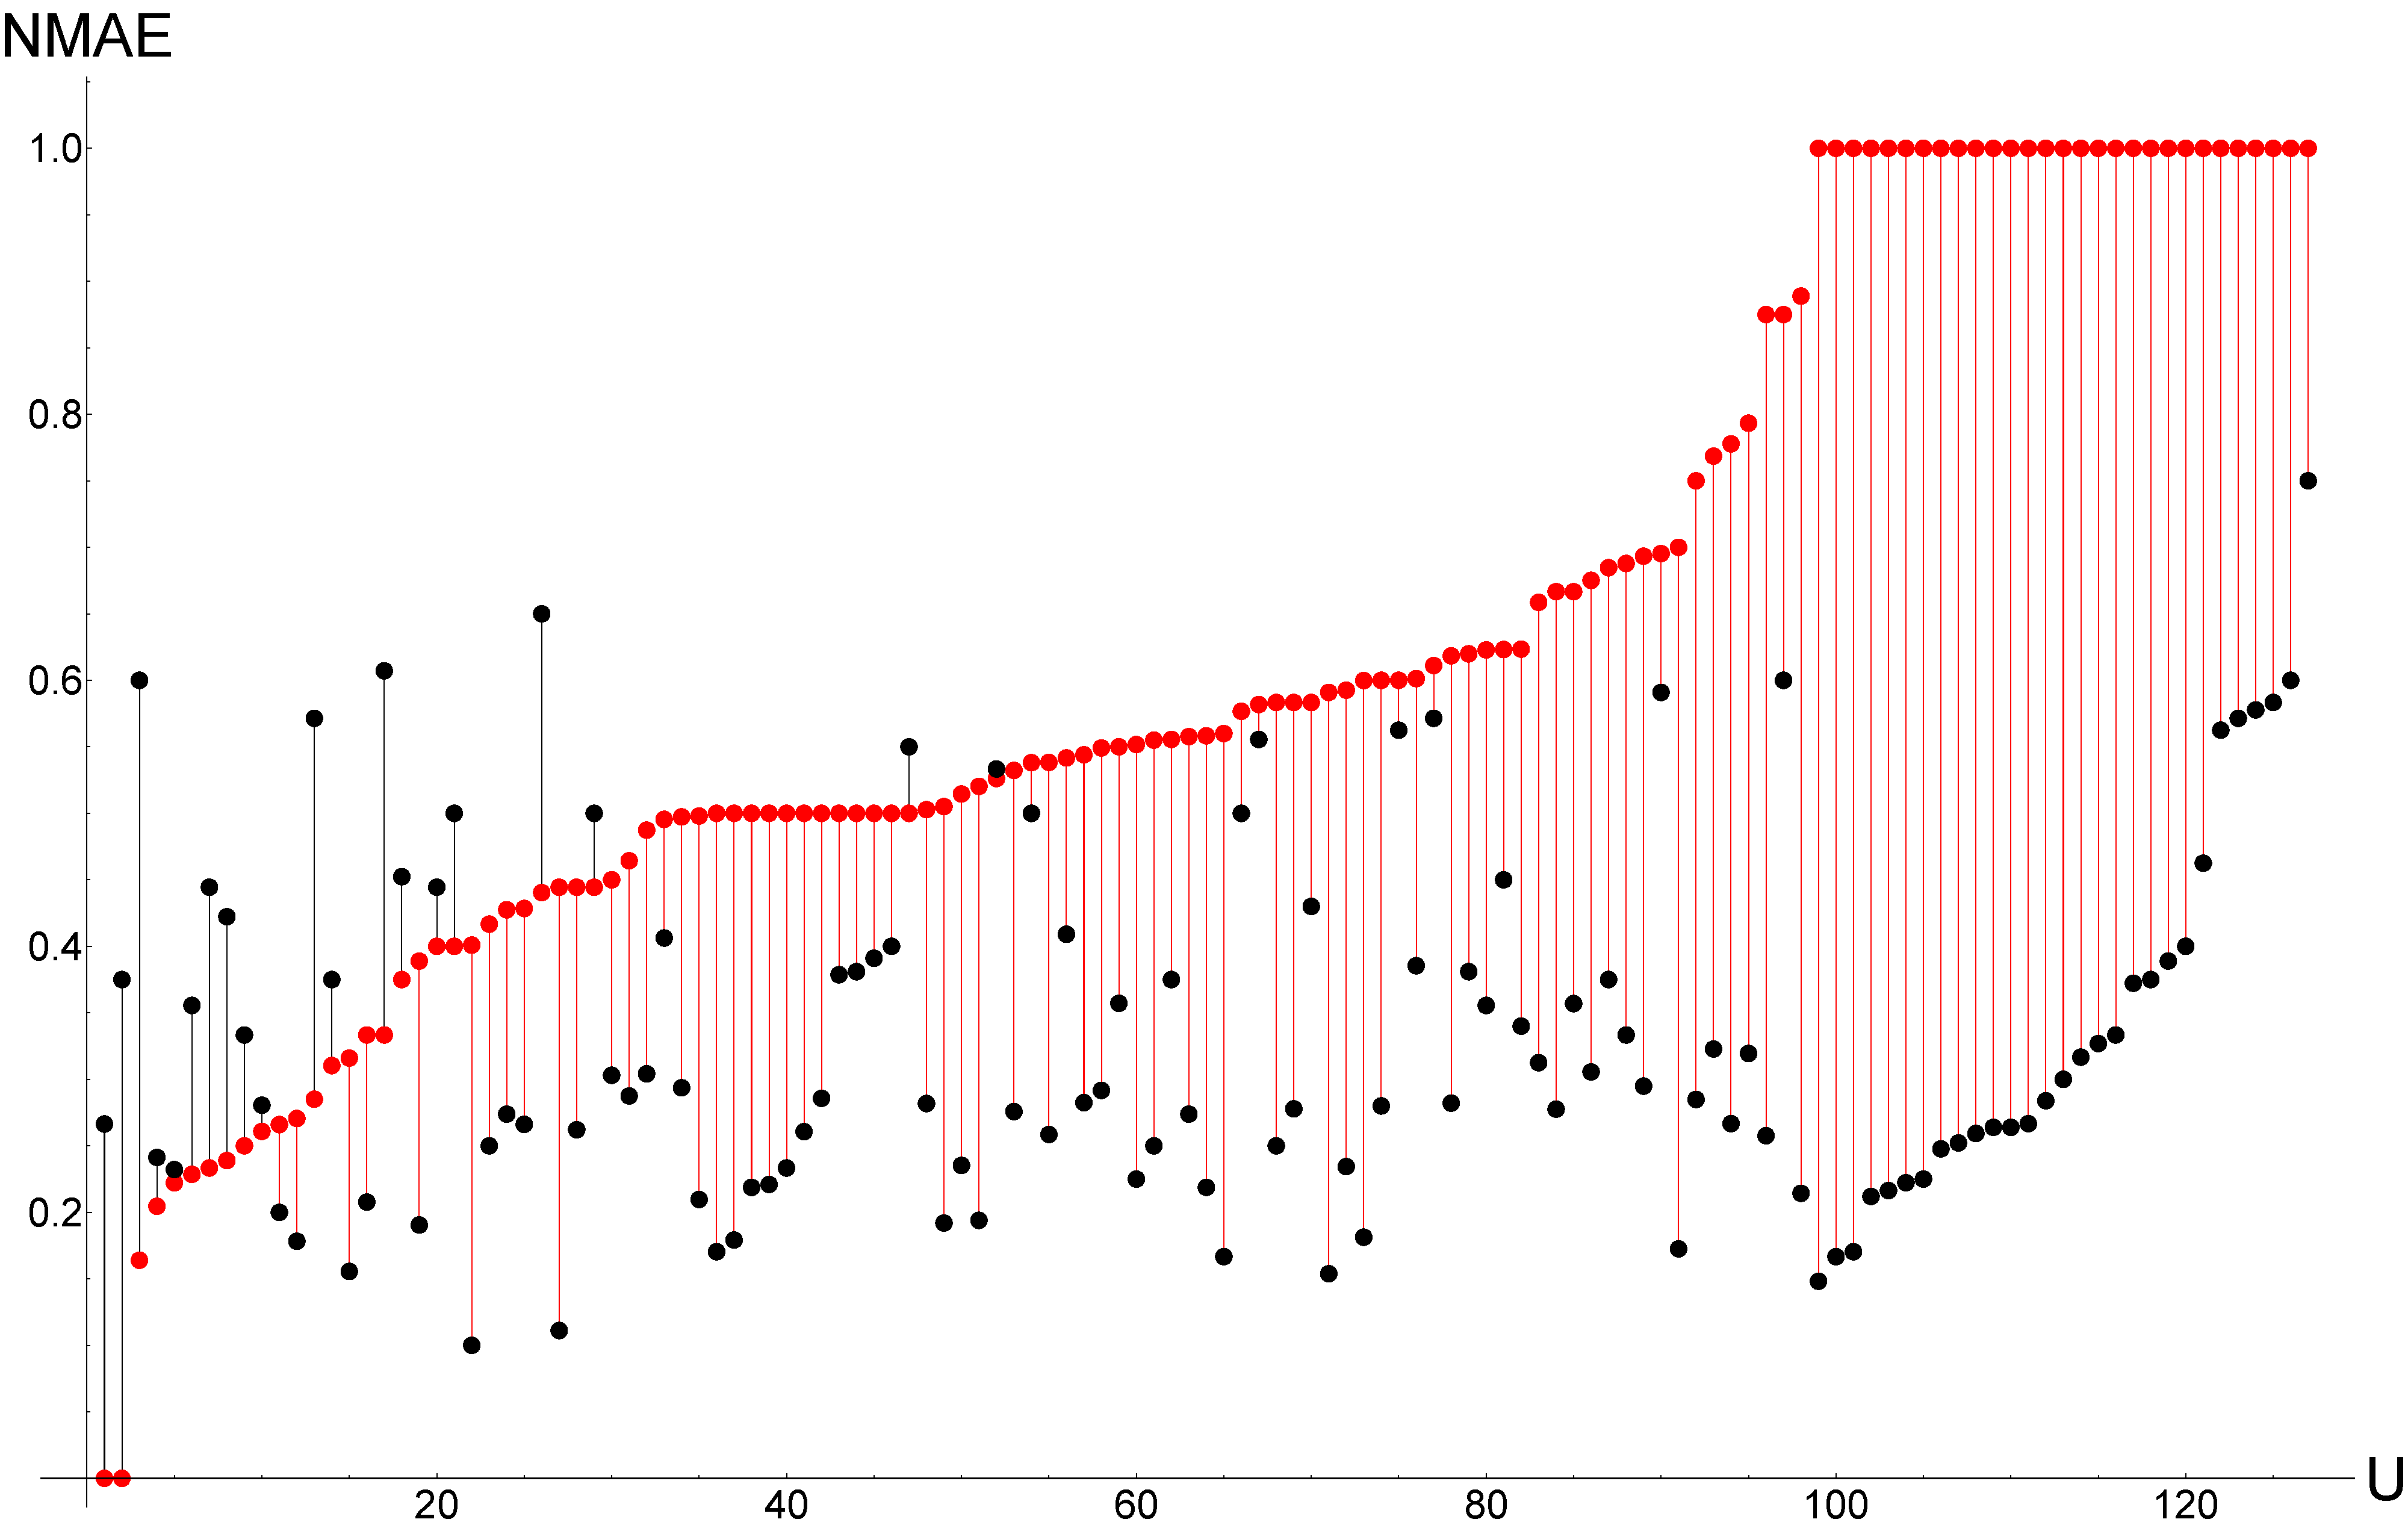
\includegraphics[width=5in,height=2in]{pics/results/ub_vs_fuzzy.pdf}
\end{center}
\end{figure}
Видно, что в большинстве НРС более эффективна по критерию качества,
в других ситуациях предпочтения пользователя неоднородны.
и эвристическое предположение, на котором основано построение
функции $\delta_c$, не верно для пользователя.

%{\bf Влияние свойства неоднородности на качество решения задачи $topN$ в ООМ и
%нечеткой модели}
%На Рис. \ref{pic:topn_trans} приведены результаты решений задачи $topN$ при
%применении $\Pi_O$ в ООМ и $\Pi_f$ и в нечеткой модели. Видно, что 
%
%\begin{figure}[htb]
%	\caption{Влияние свойства транзитивности на ООМ при решении задачи $topN$}
%	\label{pic:topn_trans}
%	\begin{center}
%		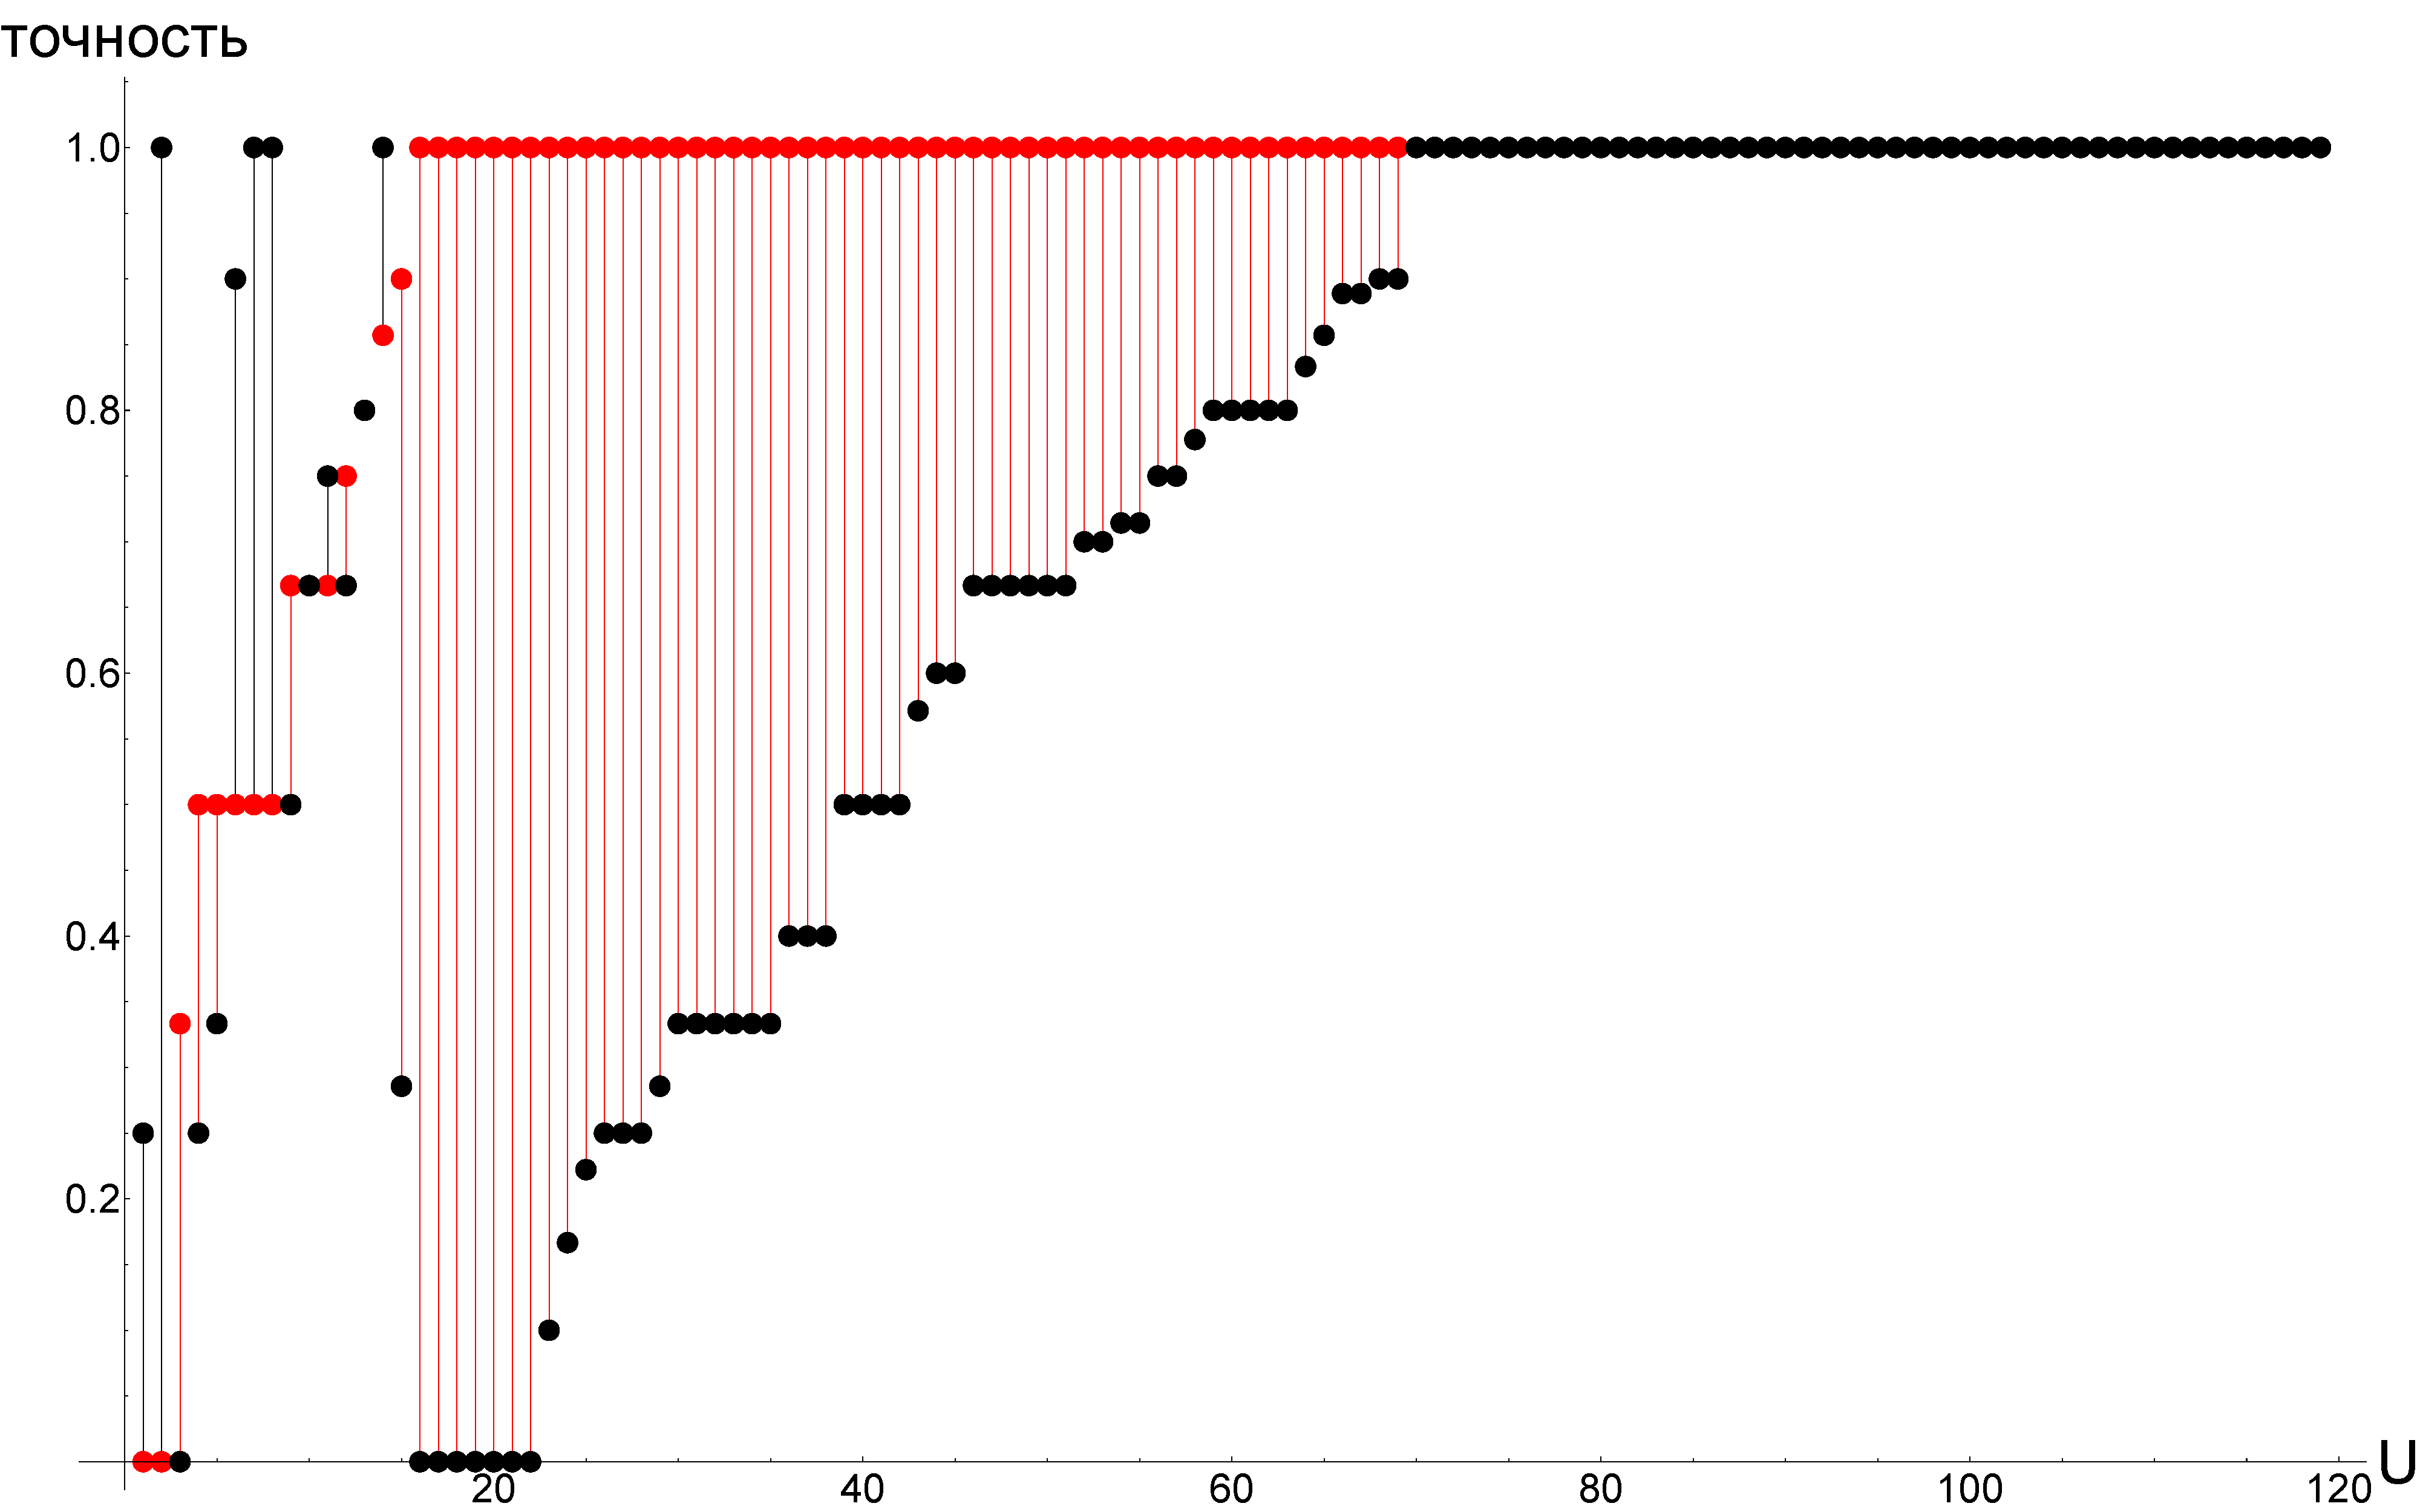
\includegraphics[width=5in,height=2in]{pics/results/transitivity.pdf}
%\end{center}
%\end{figure}



%\subsubsection{Влияние свойства транзитивности}
%В главе, посвященной анализу АКМ было выведено достаточное (\ref{suf-cond-pred-srs}) и
%необходимое (\ref{nec-cond-pred-srs})
%условие, при выполнении которого АКМ гарантируют получение эффективного
%решения. Это условие заключается в том, что на кластере соседей
%должно выполняться свойство транзитивности отношения близости.
%При применении нечеткой модели достаточное и необходимое условия выполняются,
%поэтому результаты решения в ней более эффективны, чем в СОМ.
%
%Выполнение свойства транзитивности зависит от того,
%какая функция используется в качестве меры сходства и какое пороговое
%значение установлено. Проведем следующие тесты:
%
%\begin{enumerate}
%	\item в СОМ при применении стандартного алгоритма решения задачи
%		прогнозирования (\ref{alg:p-srs}), основанного на
%		правиле вывода $\Pi_C$. Пороговое значение $\Delta_u$ равно $0,1$,
%		применяемая мера сходства --- коэффициент корреляции Пирсона
%		(\ref{pearson});
%
%	\item  в СОМ при применении стандартного алгоритма решения задачи
%		прогнозирования (\ref{alg:p-srs}), основанного на
%		правиле вывода $\Pi_C$. Пороговое значение $\Delta_u$ равно $0,5$,
%		применяемая мера сходства --- коэффициент корреляции Пирсона
%\end{enumerate}
%
%Результаты представлены таблицей <<Среднее значение $NMAE$ при различных пороговых значения>> (\ref{tbl:trans-p}), в которой
%указаны средние значения для $NMAE$ по всем пользователям. Среднее значение
%$NMAE$ при использовании $\Delta = 0,1$ на порядок ниже, чем значение
%$NMAE$ при использовании $\Delta = 0,5$.
%Так как при использовании коэффициента корреляции Пирсона,
%если $(\du(u, v) = 1) \wedge (\du(v, z) = 1) \Rightarrow (\du(u, z) =
%1)$, то при пороговом значении $\Delta_u = 0,1 $вероятность того,
%что свойство транзитивности на кластере соседей будет проявляться,
%выше, чем при использовании $\Delta_u = 0,5$.
%
%Практические результаты подтверждают теоретический вывод
%(\ref{suf-cond-pred-srs}, \ref{nec-cond-pred-srs}) о том, что
%от выполнения свойства транзитивности отношения близости зависит
%качество решения задачи прогнозирования в СОМ, а
%выполнение свойства транзитивности зависит от таких параметров,
%как функция, используемая в качестве меры сходства и ее порогового
%значения.
%
%\begin{table}[htb]
%	\caption{Среднее значение $NMAE$ при различных пороговых значения}
%  \begin{center}
%	\label{tbl:trans-p}
%	\begin{tabular}{|c|c|}
%	  \hline
%		Пороговое значение & NMAE \\ \hline
%		0,1&0,495 \\ \hline
%		0,5&0,601 \\ \hline
%	\end{tabular}
%  \end{center}
%\end{table}


%
% =============== OLD ==============
%


%Для решения задач $topN$ и прогнозирования в ООМ и СОМ соответственно
%использовались стандартные алгоритмы и подходы, которые заключаются
%в построении кластера соседей. При решении задачи $topN$ в
%ООМ использовалась мера сходства косинус, при решении задачи прогнозирования
%в СОМ – коэффициент корреляции Пирсона. Те же алгоритмы были применены при
%решении задач в нечеткой модели, но при этом использовались
%расстояния $\rhi$ и $\rhu$ и описанные выше модификации алгоритмов.
%Пороговое значение $\varepsilon_p, \varepsilon_i$ было принято равным 0,1.
%
%Стандартно при проведении тестирования данные о пользователе случайно
%разбивались в следующем отношении: 80\% – обучающее множество,
%20\% – тестовое. Обозначим такое разбиение цифрой 1. Помимо стандартного
%разбиения использовались и другие специально сформированные разбиения 2 и 3.
%Разбиение 2 составлено так, что обучающее множество состоит из таких объектов
%$i$,  для которых выполняется отношение $\rt$, тестовое множество состоит из
%таких объектов $j$, для которых отношение $i \rt j$ не выполняется.
%Такое разбиение создано для того, чтобы подтвердить или опровергнуть
%влияние свойства неоднородности данных на эффективность по критерию качества.
%Разбиение 3 составлено так же, как и стандартное разбиение, но в нем участвуют
%только те пользователи, для которых функция $\delta_c$ задана аккуратно.
%
%Эффективность решений задач по критерию качества определяется усредненными
%по числу тестов (равному 1000 для каждой задачи, разбиению и модели) значениями
%функций, использующихся в РС в качестве оценок.
%Эффективность решения задачи $topN$ по критерию качества оценивалась
%значениями функций точность (P), точность по списку длины L, средняя точность,
%NDCG.
%В результате тестирования среднее значение этих функций мало отличалось,
%поэтому в Таблице \ref{table:topn} приведены только значения точности.
%Большее значение
%точности свидетельствует о то, что решение более эффективно. Эффективность
%решения задачи прогнозирования по критерию качества оценивалась значениями
%функций MAE, NMAE, RMSE, меньшее значение которых говорит о более эффективном
%решении.
%В результате тестирования среднее значение этих функций мало отличалось,
%поэтому в Таблице \ref{table:p} приведены только значения NMAE.
%
%\begin{table}[htb]
%	\caption{Задача $p$}
%  \begin{center}
%	\label{table:p}
%	\begin{tabular}{|c|c|c|c|}
%	  \hline
%		\textnumero & Модель/Правило вычисления & Разбиение & P \\ \hline
%		1&СОМ/$\Pi_{COM}$&1&0,23 \\ \hline
%		2&СОМ/$\Pi_{COM}$&2&0,21 \\ \hline
%		3&Нечеткая СОМ/$\Pi_{COM}$&1&0,13 \\ \hline
%		4&Нечеткая СОМ/$\Pi_{COM}$&2&0,18 \\ \hline
%		5&Нечеткая СОМ/$\Pi_{f}$&1&0,21 \\ \hline
%		6&Нечеткая СОМ/$\Pi_{f}$&2&0,22 \\ \hline
%		7&Нечеткая СОМ/$\Pi_{f}$&3&0,11 \\ \hline
%		8&СОМ$^{\star}$/$\Pi_{COM}$&2&0,15 \\ \hline
%	\end{tabular}
%  \end{center}
%\end{table}
%
%\begin{table}[htb]
%	\caption{Задача $topN$}
%  \begin{center}
%	\label{table:topn}
%	\begin{tabular}{|c|c|c|c|}
%	  \hline
%		\textnumero & Модель/Правило вычисления & Разбиение & NMAE \\ \hline
%		1&ООМ/$\Pi_{OOM}$&1&0,32 \\ \hline
%		2&ООМ/$\Pi_{OOM}$&2&0,24 \\ \hline
%		3&Нечеткая ООМ/$\Pi_{OOM}$&1&0,55 \\ \hline
%		4&Нечеткая ООМ/$\Pi_{OOM}$&2&0,53 \\ \hline
%		5&Нечеткая ООМ/$\Pi_{f}$&1&0,39 \\ \hline
%		6&Нечеткая ООМ/$\Pi_{f}$&2&0,36 \\ \hline
%		7&Нечеткая ООМ/$\Pi_{f}$&3&0,81 \\ \hline
%	\end{tabular}
%  \end{center}
%\end{table}
%
%Прокомментируем данные Таблиц \ref{table:topn} и \ref{table:p}. Результаты 1 эффективней результатов 2 и
%результаты 3 эффективней результатов 4, что подтверждает теоретические выводы
%о влиянии свойства неоднородности на эффективность по критерию качества при
%применении ООМ. Разбиение 2 задано так, что свойства неоднородности влияют на
%эффективность решения, так как между объектами обучающего и тестового
%множеств не выполняется отношение сходства, в результате чего нарушается
%утверждение ООМ (\ref{ors-assert}). Разбиение 2 увеличивает вероятность того, что утверждение
%СОМ (\ref{srs-assert}) может быть неверным, поэтому результаты 1 и 3
%эффективней результатов 2 и 4 Таблицы 2.
%Результаты 3 и 4 эффективней результатов 1 и 2, что подтверждает вывод о том,
%что нечеткая контентная модель является эффективным расширением, так как в
%ней выполняются
%достаточные условия
%1 и 2. Эти же результаты подтверждают выводы о влиянии меры сходства на
%эффективность ООМ и СОМ по критерию качества.
%Результаты 7 эффективней результатов 3–6, так как для разбиения 7 функция
%$\delta_c$
%задана аккуратно. Результаты 7 эффективней результатов 5 и 6, так как для 5 и 6
%в общем случае $\delta_c$  не задана аккуратно, и поэтому же 5 и 6 не
%эффективней 3 и 4. Результаты 5 эффективней 6, так как функция $\delta_c$
%задавалась на основании данных обучающего множества, и поэтому свойство
%неоднородности влияет на аккуратность функции так же, как и на эффективность
%КМ по критерию качества. Использование
%$\Pi_f$ может быть неэффективным, если о пользователях известна только та
%информация, которая
%принадлежит исходному множество P. В такой ситуации эффективней использовать
%нечеткую модель
%$\Pi_{OOM}$ или $\Pi_{COM}$. Для задания функции $\delta_c$ можно использовать
%информацию, которая никак не зависит
%от мощности и свойств исходных данных, и тогда решения задач в нечеткой
%контентной модели не будут
%зависеть от свойств исходных данных. Такой информацией может выступать, к примеру, контекстная информация
%
%Результаты 8 эффективней результатов 1 --- в этом тесте использовался
%модифицированный алгоритм построения кластера соседей\ref{method}.
%Данный результат является следствием того, что на построенном кластере
%выполняется достаточное условие получения эффективного решения по критерию
%качества.
%



\underline{\bf Выводы}
В ходе диссертационного исследования были решены поставленные задачи.
\begin{enumerate}
	\item заданы критерии оценки качества моделей РС;
	\item проведен анализ качества АКМ по
		заданным критериям, в результате чего определены достаточные условия, при
		выполнении которых АКМ гарантируют получение
		качественного решения, и показано, что в общем
		случае АКМ не являются качественными моделями;
	\item определена математическая модель НРС, в которой:
		\begin{enumerate}
			\item методы решений задач АКМ дают более высокое качество,
				что достигается за счет выполнения выведенных
				достаточных условий в НРС;

			\item разработан формальный способ определения прогнозной функции
				$\rh$, основанный на введении нечеткого отображения
				$\Psi: U \rightarrow I$;

			\item разработаны алгоритмы решения задач, обладающие меньшей
				асимптотической сложностью по сравнению с алгоритмами
				решений, используемыми в АКМ.
				Разработанные алгоритмы будут гарантировать качественное
				решение независимо от таких дополнительных условий,
				как свойства исходных данных и выполнение
				эвристических утверждений. Разработанные алгоритмы обладают
				большее высоким качеством, чем алгоритмы
				АКМ;

		\end{enumerate}
	\item разработано ПО для проведения тестирования;
	\item проведено тестирование, результаты которого подтверждают
		теоретические выводы.
\end{enumerate}

Опубликованные статьи:
\begin{enumerate}
% печатный
\item Понизовкин Д. М.
Оптимальное распределение проектов при проведении экспертизы / Д. М. Понизовкин, С. А. Амелькин //
Электронные библиотеки: Перспективные Методы и Технологии,
Электронные коллекции. --- 2010. --- С. 524-525.
% электронный, ВАК
\item Понизовкин Д. М. Построение оптимального графа связей в системах коллаборативной фильтрации / Д. М. Понизовкин, С. А. Амелькин //
Программные системы: теория и приложения. 2011.--- Т. 2. --- № 4. С. 107–114
% электронный, ВАК
\item Понизовкин Д. М. Математическая модель коллаборативных процессов принятия решений //
Программные системы: теория и приложения. 2011. --- Т. 2. --- № 4. С 95-99.
% электронный
\item Амелькин С. А, Д. М. Понизовкин. Оптимальное проведение экспертизы образовательных процессов / С. А. Амелькин, Д. М. Понизовкин //
Труды XVII Всероссийской научно-методической конференции Телематика’2010,
Санкт-Петербург: Университетские телекоммуникации. --- 2010. ---
Т. 1, С. 158-159.
% электронный, ВАК
\item Д. М. Понизовкин. Влияние меры сходства на результативность РС // Программные системы: теория и приложения, 2014. --- Т. 2. --- N. 5. С 55–65.
% печатный, ВАК
\item С. А. Амелькин, Д. П. Понизовкин. Математическая модель задачи $topN$ для
	контентных рекомендательных систем //
Известия МГТУ МАМИ, Т. 2 , c. 26–31

% Печатный, ВАК
\item Д. М. Понизовкин.
	Повышение качества решения задачи $topN$ коллаборативными рекомендательными
	системами
	//
	Современная наука: актуальные проблемы теории и практики.
	Серия естественные и технические науки. 2017 ---
	Т. 7-8. --- с 62-67.
% Электронный web of science
\item Д. М. Понизовкин.
		Модель рекомендательной системы на нечетких множествах
		как эффективное расширение коллаборативной модели//
		Data Analytics and Management in Data Intensive Domains:
		Collection of Scientific Papers of the XIX International
		Conference DAMDID / RCDL’2017 (October 10–13, 2017, Moscow, Russia),
		2017. - c 118-123/
\end{enumerate}

\end{document}

